\documentclass[12pt, dvipsnames]{report}

\usepackage{amsmath}
\usepackage{algorithm}
%\usepackage{algorithmic}
\usepackage[noend]{algpseudocode}

\usepackage{amsmath}
\usepackage{amssymb}
\usepackage{amsthm}
\usepackage{amsopn}

\usepackage{kpfonts}

\usepackage{graphicx}

% Probably don't need this on notes anymore
%\usepackage{kbordermatrix}

% Standard tool for drawing diagrams.
\usepackage{tikz}
\usepackage{tkz-berge}
\usepackage{tikz-cd}
\usepackage{tkz-graph}

\usepackage{comment}

%
\usepackage{multicol}

%
\usepackage{framed}

%
\usepackage{mathtools}

%
\usepackage{float}

%
\usepackage{subfig}

%
\usepackage{wrapfig}

%
\let\savewideparen\wideparen
\let\wideparen\relax
\usepackage{mathabx}
\let\wideparen\savewideparen

% Used for generating `enlightening quotes'
\usepackage{epigraph}

% Forget what this is used for :P
\usepackage[utf8]{inputenc}

% Used for generating quotes.
\usepackage{csquotes}

% Allows what to generate links inside
% generated pdf files
\usepackage{hyperref}

% Allows one to customize theorem
% environments in mathematical proofs.
\usepackage{thmtools}

% Gives access to a proof
\usepackage{lplfitch}

% I forget what this is for.
\usepackage{accents}

% A package for drawing simple trees,
% as a substitute for unnesacary TIKZ code
\usepackage{qtree}

% Enables sequent calculus proofs
\usepackage{ebproof}

% For braket notation
\usepackage{braket}

% To change line spacing when using mathematical notations which require some height!
\usepackage{setspace}

%\usepackage[dvipsnames]{xcolor}

\usepackage{float}

% For block commenting
\usepackage{comment}




\setlength\epigraphwidth{8cm}

\usetikzlibrary{arrows, petri, topaths, decorations.markings}

% So you can do calculations in coordinate specifications
\usetikzlibrary{calc}
\usetikzlibrary{angles}

\theoremstyle{plain}
\newtheorem{theorem}{Theorem}[chapter]
\newtheorem{axiom}{Axiom}
\newtheorem{lemma}[theorem]{Lemma}
\newtheorem{corollary}[theorem]{Corollary}
\newtheorem{prop}[theorem]{Proposition}
\newtheorem{exercise}{Exercise}[chapter]
\newtheorem{fact}{Fact}[chapter]

\newtheorem*{example}{Example}
\newtheorem*{proof*}{Proof}

\theoremstyle{remark}
\newtheorem*{exposition}{Exposition}
\newtheorem*{remark}{Remark}
\newtheorem*{remarks}{Remarks}

\theoremstyle{definition}
\newtheorem*{defi}{Definition}

\usepackage{hyperref}
\hypersetup{
    colorlinks = true,
    linkcolor = black,
}

\usepackage{textgreek}

\makeatletter
\renewcommand*\env@matrix[1][*\c@MaxMatrixCols c]{%
  \hskip -\arraycolsep
  \let\@ifnextchar\new@ifnextchar
  \array{#1}}
\makeatother

\renewcommand*\contentsname{\hfill Table Of Contents \hfill}

\newcommand{\optionalsection}[1]{\section[* #1]{(Important) #1}}
\newcommand{\deriv}[3]{\left. \frac{\partial #1}{\partial #2} \right|_{#3}} % partial derivative involving numerator and denominator.
\newcommand{\lcm}{\operatorname{lcm}}
\newcommand{\im}{\operatorname{im}}
\newcommand{\bint}{\mathbf{Z}}
\newcommand{\gen}[1]{\langle #1 \rangle}

\newcommand{\End}{\operatorname{End}}
\newcommand{\Mor}{\operatorname{Mor}}
\newcommand{\Id}{\operatorname{id}}
\newcommand{\visspace}{\text{\textvisiblespace}}
\newcommand{\Gal}{\text{Gal}}

\newcommand{\xor}{\oplus}
\newcommand{\ft}{\wedge}
\newcommand{\ift}{\vee}

\newcommand{\prob}{\mathbf{P}}
\newcommand{\expect}{\mathbf{E}}
\DeclareMathOperator{\Var}{\mathbf{V}}
\newcommand{\Ber}{\text{Ber}}
\newcommand{\Bin}{\text{Bin}}

%\newcommand{\widecheck}[1]{{#1}^{\ft}}

\DeclareMathOperator{\diam}{\text{diam}}

\DeclareMathOperator{\QQ}{\mathbf{Q}}
\DeclareMathOperator{\ZZ}{\mathbf{Z}}
\DeclareMathOperator{\RR}{\mathbf{R}}
\DeclareMathOperator{\HH}{\mathbf{H}}
\DeclareMathOperator{\CC}{\mathbf{C}}
\DeclareMathOperator{\AB}{\mathbf{A}}
\DeclareMathOperator{\PP}{\mathbf{P}}
\DeclareMathOperator{\MM}{\mathbf{M}}
\DeclareMathOperator{\VV}{\mathbf{V}}
\DeclareMathOperator{\TT}{\mathbf{T}}
\DeclareMathOperator{\LL}{\mathcal{L}}
\DeclareMathOperator{\EE}{\mathbf{E}}
\DeclareMathOperator{\NN}{\mathbf{N}}
\DeclareMathOperator{\DQ}{\mathcal{Q}}
\DeclareMathOperator{\IA}{\mathfrak{a}}
\DeclareMathOperator{\IB}{\mathfrak{b}}
\DeclareMathOperator{\IC}{\mathfrak{c}}
\DeclareMathOperator{\IP}{\mathfrak{p}}
\DeclareMathOperator{\IQ}{\mathfrak{q}}
\DeclareMathOperator{\IM}{\mathfrak{m}}
\DeclareMathOperator{\IN}{\mathfrak{n}}
\DeclareMathOperator{\IK}{\mathfrak{k}}
\DeclareMathOperator{\ord}{\text{ord}}
\DeclareMathOperator{\Ker}{\textsf{Ker}}
\DeclareMathOperator{\Coker}{\textsf{Coker}}
\DeclareMathOperator{\emphcoker}{\emph{coker}}
\DeclareMathOperator{\pp}{\partial}
\DeclareMathOperator{\tr}{\text{tr}}

\DeclareMathOperator{\supp}{\text{supp}}

\DeclareMathOperator{\codim}{\text{codim}}

\DeclareMathOperator{\minkdim}{\dim_{\mathbf{M}}}
\DeclareMathOperator{\hausdim}{\dim_{\mathbf{H}}}
\DeclareMathOperator{\lowminkdim}{\underline{\dim}_{\mathbf{M}}}
\DeclareMathOperator{\upminkdim}{\overline{\dim}_{\mathbf{M}}}
\DeclareMathOperator{\lhdim}{\underline{\dim}_{\mathbf{M}}}
\DeclareMathOperator{\lmbdim}{\underline{\dim}_{\mathbf{MB}}}
\DeclareMathOperator{\packdim}{\text{dim}_{\mathbf{P}}}
\DeclareMathOperator{\fordim}{\dim_{\mathbf{F}}}

\DeclareMathOperator*{\argmax}{arg\,max}
\DeclareMathOperator*{\argmin}{arg\,min}

\DeclareMathOperator{\ssm}{\smallsetminus}

\title{Algebraic Geometry}
\author{Jacob Denson}

\begin{document}

\pagenumbering{gobble}
\maketitle
\tableofcontents
\pagenumbering{arabic}

\chapter{Affine Algebraic Sets}

\section{Planar Algebraic Curves}

Classically, Euclidean geometry discusses the relations between the intersections of lines and circles. However, this geometry has proved inadequete for certain constructions. For instance, one cannot use lines and circles to construct a cube with twice the volume of another cube. Similarily, one cannot trisect general angles, nor . However, by introducing more complicated geometric shapes, one is able to solve these problems. The Greek mathematician Menaechmus introduced the parabola to square the circle. Pappus used the hyperbola to trisect the angle. Thus the conic sections became a canonical part of Euclidean geometry. Thanks to Descartes' analytical geometry, we can identify the Euclidean plane with coordinates: tuples of two numbers. Furthermore, lines, circles, and conic sections are then described as the {\it locus} of points satisfying some algebraic relationship between the coordinates.
%
\begin{itemize}
    \item A circle is the locus of points lying at a fixed radius from a certain center point. If we consider a coordinate system where the center lies at the origin, and where the radius is a unit distance, then the points on the circle are exactly those satisfying $X^2 + Y^2 = 1$.

    \item A parabola can be described as those points whose distance to a fixed point (known as the focus) is equal to the distance between the point and a fixed line. The canonical equation for such an parabola is $Y = X^2$.

    \item A hyperbola is defined by a pair of focal points, such that the difference between the distances two the two focal points is a fixed quantity. The canonical equation for such a hyperbola is $X^2 - Y^2 = 1$.
\end{itemize}
%
An {\bf algebraic plane curve} is a geometric shape in the plane described as the locus of a polynomial equation. The techniques used to understand the algebraic curves formed the historical foundation for the study of algebraic geometry.

\begin{example}
    A cissoid is a curve obtained from two other given curves $C_1$ and $C_2$ and a pole $O$, and is the locus obtained by taking pairs of points $P_1 \in C_1$ and $P_2 \in C_2$ such that $O$ lies on $P_1P_2$, and then consdering the point $P$ on the line $P_1P_2$ such that the distance between $O$ and $P$ is equal to the distance between $P_1$ and $P_2$ (there are two such points, but $P$ is chosen so that $OP$ is oriented the same as $P_1P_2$ on the line.

    \begin{center}
    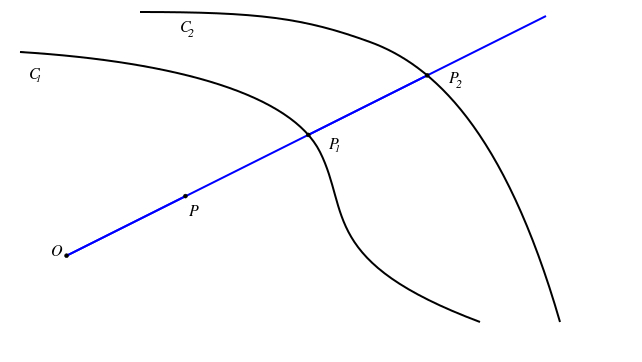
\includegraphics[width=0.6\textwidth]{cissoidconstruction.jpg}
    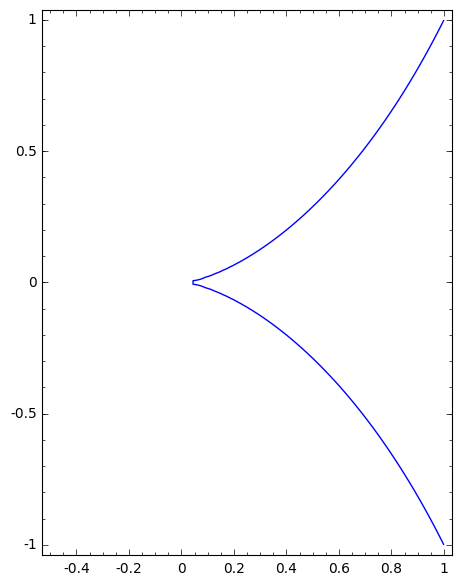
\includegraphics[width=0.3\textwidth]{cissoid}
    \end{center}

    The {\bf cissoid of Diocles} is obtained by taking $C_1$ to be a circle, $C_2$ a line tangent to the circle, and $O$ the point opposite the tangent line. In this case, we can also describe the cissoid as those points obtained by taking a point $P$ on the circle, and considering the intersection of the line $OP$ with the line parallel to the tangent at $O$ through the point $Q$ obtained by reflecting $P$ about the line parallel to the tangent which bisects the circle. This claim is proved by a simple geometric argument (similarity of triangles) suggested by the diagram below.

    \begin{center}
        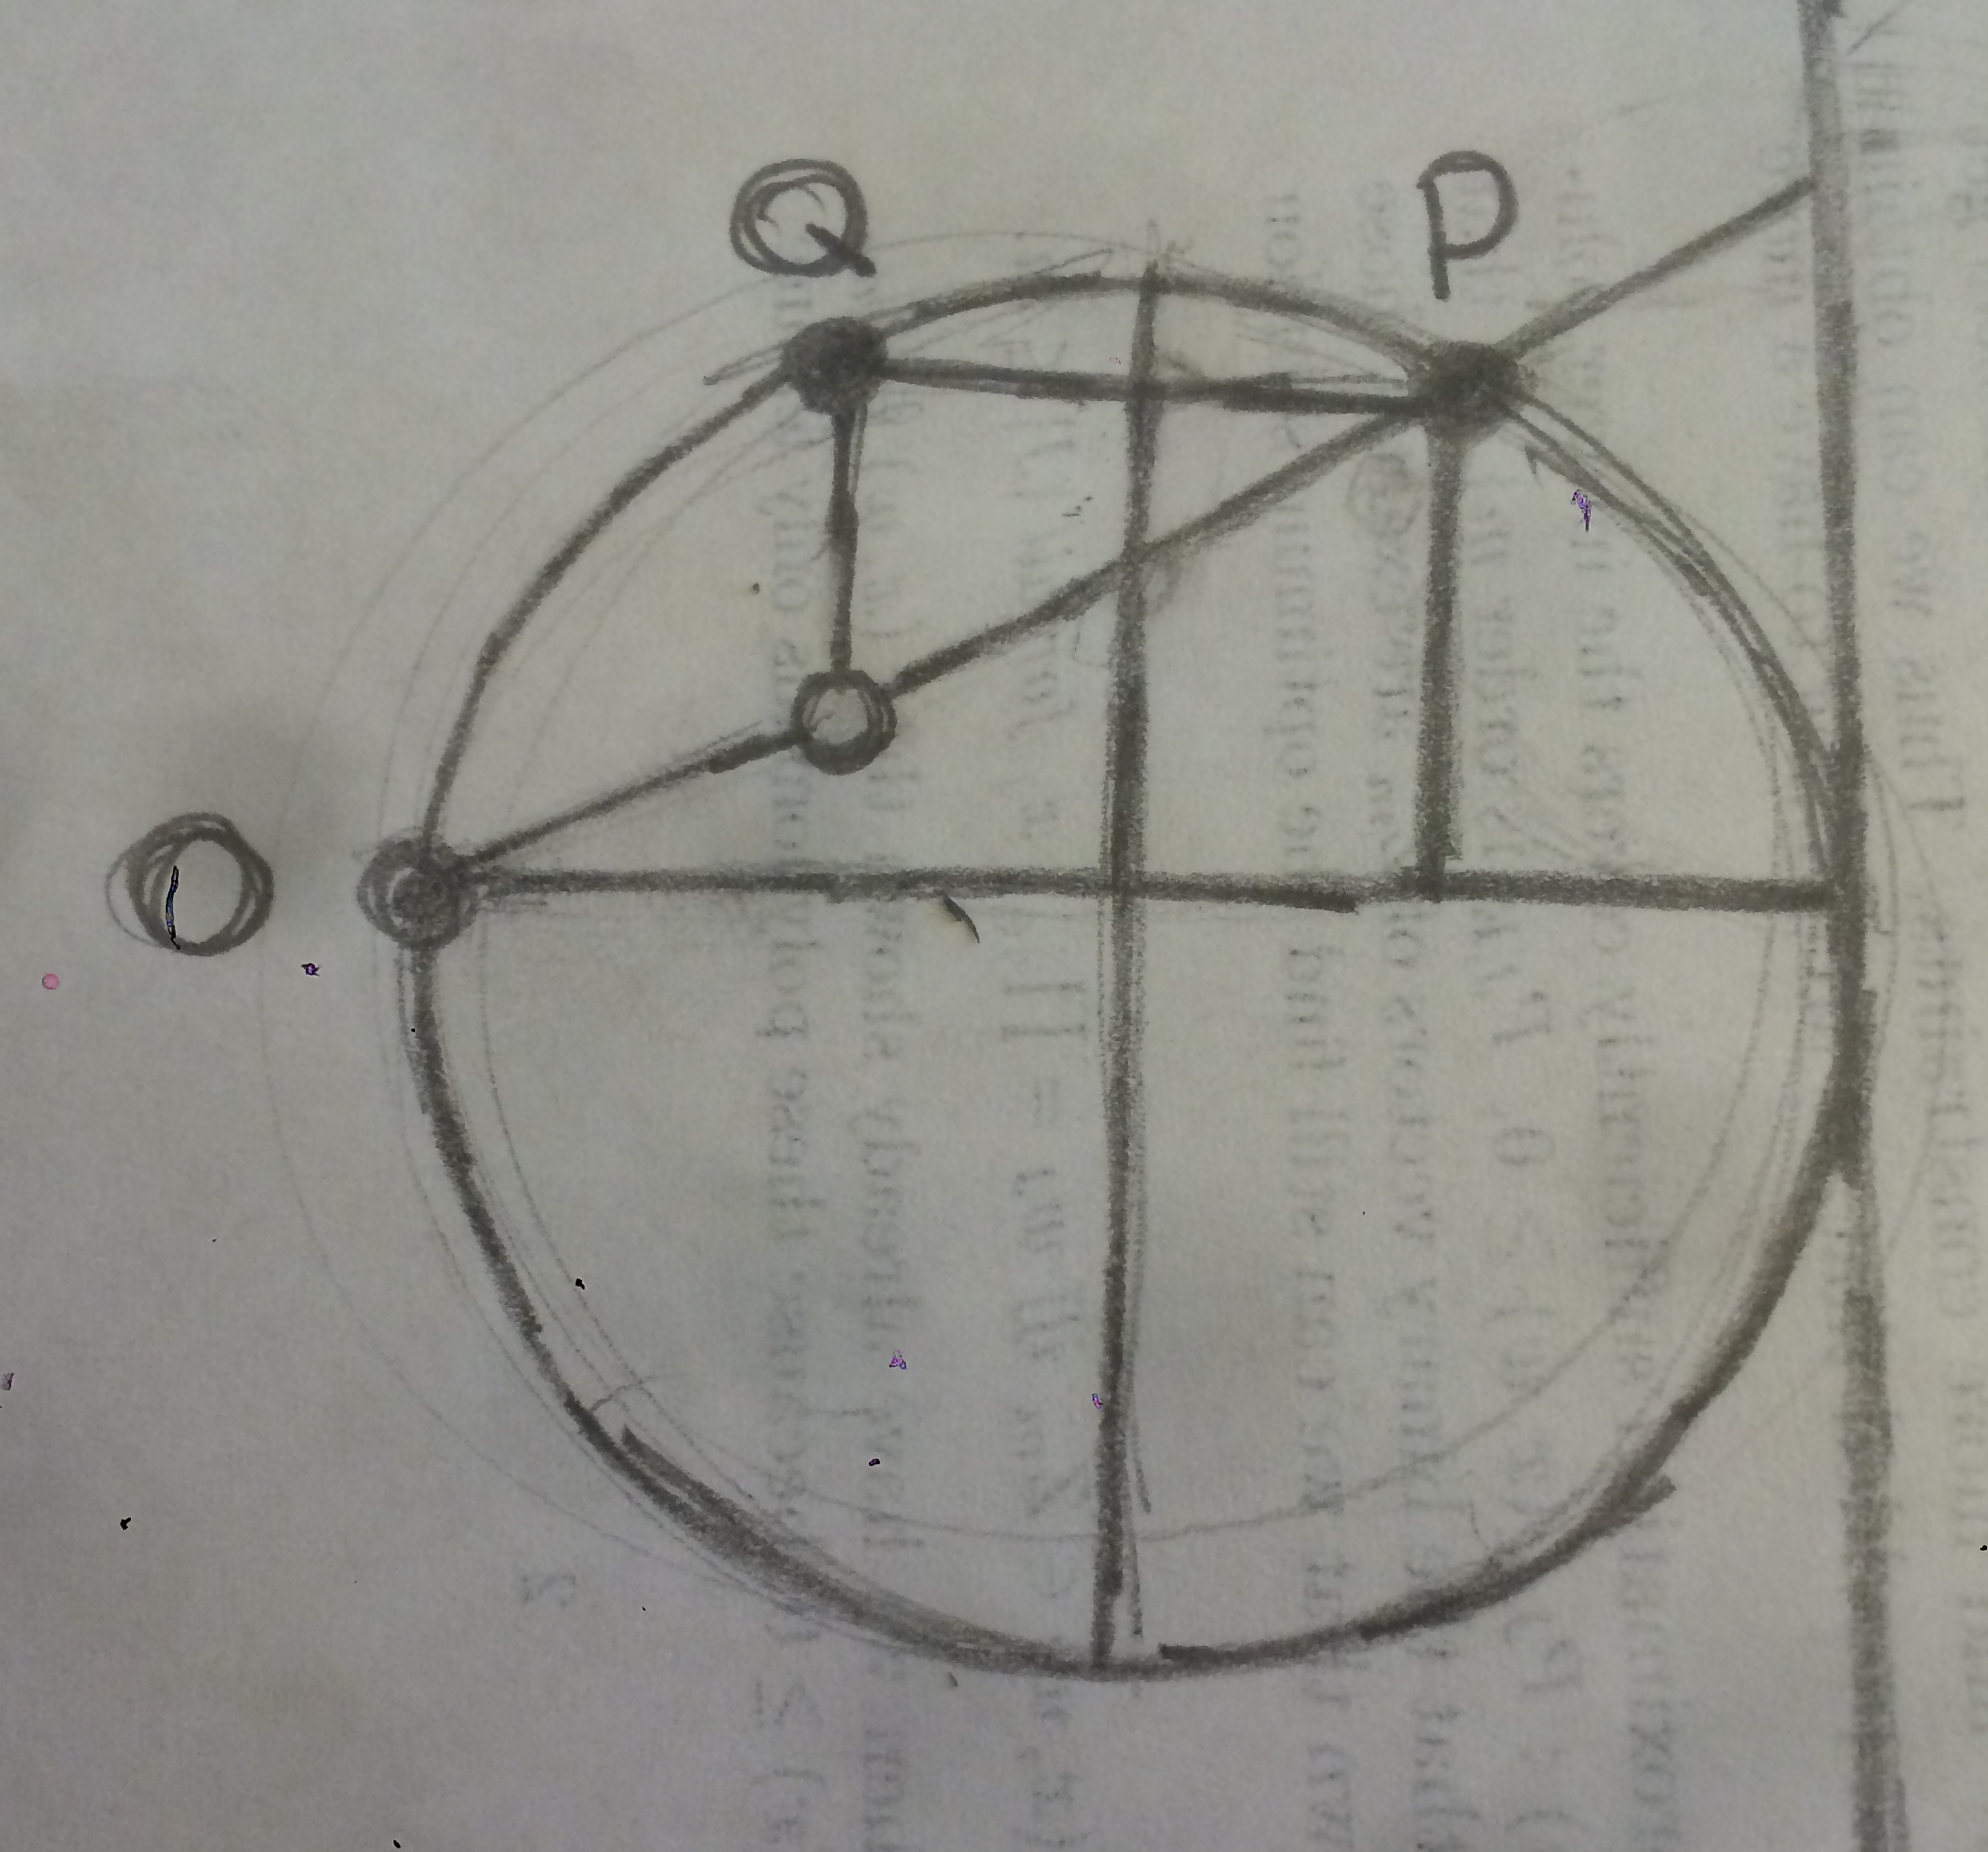
\includegraphics[width=0.4\textwidth]{cissoidreflect.jpg}
    \end{center}

    If we consider a coordinate system in which $O$ lies at the origin, $C_1$ is the unit circle with center $(1,0)$, and $C_2$ is the line $X = 2$, then in polar coordinates, we may write the points on $C_1$ as the solutions to $r = 2 \sec t$, and the points on $C_2$ by $r = 2 \cos t$. The advantage of these coordinates is that the angles $t$ parameterize the lines through $O$, and thus the intersection points $P_1$ and $P_2$ on the individual curves. The distance between the line $r = 2 \sec t$ and $r = 2 \cos t$ is equal to the difference in radii between the two curves at the point, so the length of the radius takes the form $2 \sec t - 2 \cos t$, and therefore the polar equation defining cissoid of Diocles is
    %
    \[ r = 2 \sec t - 2 \cos t = \frac{2 - 2\cos^2 t}{\cos t} = \frac{2 \sin^2 t}{\cos t}\]
    %
    Since $X = r \cos t$, $Y = r \sin t$, and $r^2 = X^2 + Y^2$, this equation can be rewritten as
    %
    \[ X = 2 \sin^2 t = \frac{2Y}{X^2 + Y^2} \]
    %
    so the cissoid of Diocles is obtained from the equation $(X^2 + Y^2) X = 2Y^2$. This algebraic equation describes the curve, so the cissoid of Diocles is a planar algebraic curve. If we change the radius of the circle to be $a$, then the radii of the points in the calculation is multiplied by $a$, so we obtain the equation $(X^2 + Y^2) X = 2aY$ describing the cissoid.
\end{example}

\begin{example}
    One can also describe the cissoid of Diocles by a construction due to Newton. Let $O$ be a point, and let $P$ vary over a line not containing $O$. If we consider a point $Q$ such that $PQO$ forms a right triangle, and the distance between $P$ and $Q$ is the same as the distance between $O$ and a line, then the midpoints between $P$ and $Q$ forms Diocles' cissoid. This means we have expressed Diocles' cissoid as a conchoid (actually, a single branch of a conchoid), that is, as a curve defined as a locus between a point $O$ and a curve $C$, which are the set of points on the lines through $O$ and a point on $C$ which lie at a fixed distance from the curve (in this case, the curve is a single line, and the distance is half the distance between the point and the line). If we choose a coordinate system in which $O = (-1,0)$, and the line over which $P$ varies is $X = 1$. For help, let $R = (1,0)$. Let $t$ be the angle $QOR$. This is equal to the angle $QPR$. If the midpoint of the line $PQ$ is $S$, which has coordinates $(x,y)$, then the distance between $S$ and $P$ is $1$, so the distance between $S$ and the line $X = 1$ is $\sin t$, and so $x = 1 - \sin t$. Since $SQ$ is length 1, we find that the $y$ coordinate of $(x,y)$ is equal to one if we rotate the plane about $O$ by an angle of $t$ anticlockwise, so $(x + 1) \sin t + y \cos t = 1$, and so we obtain the parameteric equations
    %
    \[ \left( 1 - \sin t, \frac{1 - (2 - \sin t) \sin t}{\cos t} \right) = \left( 1 - \sin t, \frac{(1 - \sin t)^2}{\cos t} \right) \]
    %
    If we write $t = 90 - u$, then
    %
    \[ \left( 1 - \sin t, \frac{(1 - \sin t)^2}{\cos t} \right) = \left( 1 - \cos u, \frac{(1 - \cos u)^2}{\sin u} \right) \]
    %
    Finally, applying double angle formulas, we end up with
    %
    \begin{align*}
        \left( 1 - \cos u, \frac{(1 - \cos u)^2}{\sin u} \right) &= \left( 2 \sin^2 u/2, \frac{4 \sin^4 u/2}{2 \sin u/2 \cos u/2} \right)\\
        &= \left( 2 \sin^2 u/2, \frac{2 \sin^3 u/2}{\cos u/2} \right)
    \end{align*}
    %
    But this is exactly the parameterization of the polar equation $r = 2\sin^2(v)/\cos(v)$, where $v = u/2$, which turns into $(X^2 + Y^2) X = 2 Y^2$. The advantage of Newton's construction is that we can obtain a family of conchoidal curves (again, actually half a conchoid) which are deformations of the cissoid of Diocles, obtained by taking another point on the line between $P$ and $Q$, rather than the midpoints.
\end{example}

\begin{example}
    Another example of an algebraic plane curve is the conchoid of D\"{u}rer (which technically isn't exactly a conchoid) is obtained by taking a pair of perpendicular lines intersecting at a point $O$, considering points $Q$ and $R$ moving on these lines such that the sum of the distances from $O$ to $Q$ and $O$ to $R$ is constant, and then taking the point on $QR$ at a fixed distance from $Q$. If we take the perpendicular lines as the $X$ and $Y$ axis, with $O$ the origin, and take the sum of distances as $b$, then each point $(X,Y)$ lies on the curve if, first, it lies on a line $PQ$, where $Q = (x,0)$ and $P = (0,y)$, where $yX + xY = xy$, such that $x + y = b$, and $(X - x)^2 + Y^2 = a^2$. We can eliminate $y$ from the equation since we can write $y = b -x$, so that $(b-x)X + xY = x(b-x)$. For a fixed $X$ and $Y$, this equation is quadratic in $x$, which can be rewritten as $x^2 + bX = x(b + X - Y)$. The equation $(X - x)^2 + Y^2 = a^2$ gives $x^2 = a^2 - Y^2 - X^2 + 2xX$, hence $a^2 - Y^2 - X^2 + bX = x(b - X - Y)$, which gives
    %
    \[ (b - X - Y)x = a^2 - Y^2 - X^2 + bX \]
    %
    Finally, we obtain the constraints on $X$ and $Y$ by multiplying the equation $(b - x)X + xY = x(b - x)$ on both sides by $(b - X - Y)^2$ allows us to eliminate the remaining values of $x$, which can be rearrange to give the equation
    %
    \[ 2y^2(x^2 + y^2) + (b^2 - 3a^2)y^2 + 2a^2b(x + y) + a^2(a^2 - b^2) = a^2x^2 + 2by^2(x + y) \]
    %
    so the curve is a quartic curve. For $b = 0$, the curve becomes a pair of lines together with a circle, and if $a = 0$, we obtain two coincident straight lines.
\end{example}

\begin{example}
    The conchoid of Nicomedes is obtained by fixing a point $P$, and letting $Q$ vary over a line not containing $P$. For each $Q$, the conchoid consists of the points on the line $PQ$ at a fixed distance away from $Q$. If we choose a coordinate system where $P$ lies at $(a,0)$, $Q$ lies at $(b,0)$, and the distance parameter is $b$, then the equation describing the conchoid is $(X - a)^2(X^2 + Y^2) = b^2X^2$. The conchoids appear to take three different forms depending on the relation between the distance between $P$ and the line, and the distance defining the conchoid. If $P$ is further away than the distance defining the conchoid, then we obtain two smooth curves. If $P$ is closer than the distance defining the conchoid, then the conchoid appears to `swing' around $P$, meeting $P$ in two intersection points. If the distance to $P$ is equal to the distance defining the conchoid, then we obtain a `cusp' at $P$, where the curve appears to swing towards $P$, and then swing out giving a sharp point. An interesting feature of the conchoid is that the time for an object to reach the `bottom' of the conchoid under the influence of gravity is independent of its original starting position. Another interesting feature of the conchoid is that it consists of two separate components lying on either side of the line $X = a$, with the line as an asymptote.
\end{example}

\begin{example}
    If $C$ is a smooth curve, then the evolute of the curve is the locus of points forming the center of curvature at these points. The semi-cubical parabola is the curve obtained as an evolute of a parabola. The curvature at the point $(x,x^2)$ is $\sqrt{1 + 4x^2}$, and since the tangent to the parabola is the line $2xX - Y = x^2$, the center of curvature to the point $(x,x^2)$ is
    %
    \[ \left(\frac{x + 4x^3 - 2x}{1 + 4x^2}, \frac{x^2 + 4x^4 + 1}{1 + 4x^2} \right) \]
\end{example}

\begin{example}
    Just as we can obtain the conic sections by intersecting a cone with a parabola, the spiric sections of perseus are obtained by intersecting a plane with a torus. The general form of an equation describing a spiric section is of the form $(X^2 + Y^2)^2 = dX^2 + eY^2 + f$. A particular family of spiric sections include the Cassini curves. These can be constructed by taking two focal points $P$ and $Q$, and considering the locus of points such that the product of the distances to $P$ and to $Q$ are a fixed quantity. If we fix the focal points at $(-1,0)$ and $(1,0)$, then an equation for the Cassini curve is $(X^2 + Y^2)^2 - 2(X^2 - Y^2) + 1 = a^4$, where $a$ is the distance parameter to the curve. Cassini was an astronomer who believed the sun rotated around the earth according to these curves. The curves are smooth, except if we let the distance $a$ be equal to $1$, in which case the point $(0,0)$ is singular since the curve intersects twice here. This curve is the lemniscate of Bernoulli, described by the equation $(X^2 + Y^2)^2 = 2(X^2 - Y^2)$.
\end{example}

\begin{example}
    The folium of Descartes is the algebraic curve defined by the equation $X^3 + Y^3 = 3XY$. It's claim to fame is that was the curve that lead to the problem of implicit differentiation. In 1638, Descartes challenged Fermat to find the tangent line to the curve at any point on the circle, and with some primordial techniques of the calculus, Fermat was able to derive the tangent line at an arbitrary point.
\end{example}

\begin{example}
    If we consider a circle lying on the outside of a circle, and we fix a point on the circle as it rotates around the circle, then provided that the circumpherence of the outer circle is a rational multiple of the circumpherence of the inner circle, we obtain an algebraic curve known as an epicycloid, and the rational multiple determined the period of rotation of the circle. If the circumpherence of the inner circle is equal to the circumpherence of the outer circle, the outer circle completes a single rotation before returning to its original location, and this curve is known as a cardoid, because it has a single cusp which looks like a heart. If the outer circle has half the circumpherence as the inner circle, the outer circle rotates twice before returning to its original position, and we obtain a function with a single cusp, and we call this shape a nephroid, since the shape looks like a kidney. Similarily, the hypocycloids are obtained by revolving a circle along the interior of the circle. If we revolve the outer circle around the inner circle, we obtain a pericycloid. If we fix a general point on these circles, we obtain the trochoids.
\end{example}

\begin{example}
    The Watt curves were discovered by James Watt in his work on the steam engine. The construction is as follows. Consider a quadrilateral $ABCD$, where $A$ and $D$ are fixed points in the plane, and $B$ and $C$ can be moved on circles around $A$ and $D$ such that the length $BC$ is fixed. We obtain a Watt curve by watching the possible configurations of an arbitrary point $M$ on the line $BC$. If one takes linkages of further roads, one can generate even more complicated curves. Every finite segment of an planar algebraic curve can be obtained by some linkage of rods.
\end{example}

\begin{example}
    The Lissajous curves is the planar trajectory of a pendulum, or of a particle undergoing simple harmonic motion. Provided the harmonic motion is rational, so that the curves are closed, the curve obtained is algebraic.
\end{example}

Sometimes, algebraic plane curves do not behave like the curves we encounter in differential geometry. For instance, the equation $X^2 + Y^2 = 0$ has only a single solution $(0,0)$, and the set $\{ (0,0) \}$ does not look like a curve at all. This difficulty disappears when we study algebraic plane curves over an algebraically closed field, because $X^2 + Y^2$ factors into $(X + iY)(X - iY)$, so the solution set is the union of two planes, known as `complex lines', through the origin, so the solution set behaves locally like a two dimensional space. A two-dimensional space is `one-dimensional' over the complex numbers, so the solution set behaves like a curve.

It is natural to study algebraic plane curves over any field, since polynomial equations are inherent in every field we consider. In general, we shall assume some field $K$ is fixed, and study the $n$ dimensional affine space $\mathbf{A}^n$ over the field $K$, which can be identified with the space $K^n$ of $n$ tuples of field elements after a coordinate system is fixed. $\mathbf{A}^1$ is referred to colloquially as the affine line, and $\mathbf{A}^2$ as the affine plane. To reduce numerous difficulties with solutions to curves, we shall often assume that $K$ is an algebraically closed field, and we can obtain results over any field by embedding the field in its algebraic closure. We have seen many examples of algebraic curves obtainable 

\section{Affine Varieties}

Given a polynomial $f \in K[X_1, \dots, X_n]$, we can consider the zero set
%
\[ V(f) = \{ p \in \mathbf{A}^n : f(p) = 0 \} \]
%
which is the {\bf hypersurface} defined by $f$. We can also consider
%
\[ V(f,g) = \{ p \in \mathbf{A}^n: f(p) = 0\ \text{and}\ g(p) = 0 \} = V(f) \cap V(g) \]
%
which is the intersection of two hyperplanes, More generally, given a set $S$ of polynomials, we can consider the set $V(S)$, which consists of the points forming the set of common zeroes of all polynomials in $S$. These zero sets are called {\bf affine varieties}, and they are the main object of study in algebraic geometry.

\begin{example}
    The unit circle is the variety $V(X^2 + Y^2 - 1)$.
\end{example}

\begin{example}
    The curve consisting of the points $\{ (t,t^2,t^3): t \in K \}$ is the zero set of $V(Y^2 - X, Z - X^3)$, and is an affine variety in $\mathbf{A}^3$.
\end{example}

\begin{example}
    The set of points whose polar coordinates $(r,\theta)$ satisfy $r = \sin(\theta)$ (in addition to the point at the origin) form a variety. If these polar coordinates were induced by an affine coordinate system $(X,Y)$, then $r \sin(\theta) = Y$, and $r^2 = X^2 + Y^2$, so we may multiply the equation by $r$ to obtain the equation $X^2 + Y^2 = Y$. We find that the equation can be rearranged to $X^2 + (Y-1/2)^2 = 1/4$, so the solution set is just a circle of radius $1/2$ centered at $(0,1/2)$.
\end{example}

The class of affine varieties is interesting from the point of view of Euclidean geometry, because it is invariant under affine transformations, and many of the interesting shapes in Euclidean geometry can be identified with certain varieties through the tools of analytic geometry. If $T$ is an affine transformation on $\mathbf{A}^n$, and if we define the map $T^*: K[X_1, \dots, X_n] \to K[X_1, \dots, X_n]$ by letting $T^*f = f \circ T$, then
%
\begin{align*}
    T^{-1}(V(\mathfrak{a})) &= \{ x : (\forall f \in \mathfrak{a}: f(Tx) = 0) \}\\
    &= \{ x : (\forall f \in \mathfrak{a}: (T^*f)(x) = 0) \}\\
    &= V(T^*\mathfrak{a})
\end{align*}
%
It is easy to prove that $T^*$ preserves the degree of polynomials, which is useful to simplify calculations in certain situations. To see an example of this technique at work, let us study {\bf affine plane curves}, which are hypersurfaces in $\mathbf{A}^2$. The {\bf degree} of such a curve is the degree of the polynomial defining this hypersurface (over fields not of characteristic zero, the degree is the degree of the {\it minimal} such polynomial, since two polynomials in a finite field can have the same solution set).

\begin{theorem}
    An affine plane curve of degree $n$ intersects a line in at most $n$ places, unless the plane curve contains the entire line.
\end{theorem}
\begin{proof}
    Consider first the easy case where the line is just the $X$ axis. In this case, the zeroes of a polynomial $f(X,Y) = \sum a_{ij} X^iY^j$ which lie on the $X$ axis are in one to one correspondence with the set of solutions to the univariate polynomial $f(X,0) = \sum a_{i0} X^i$. If $f(X,0) = 0$, then $V(f)$ contains the $X$ axis, and otherwise $f$ can have at most $\deg f(X,0) \leq \deg f(X,Y) = n$ points, the intersection of $V(f)$ and the $X$ axis can contain at most $\deg f(X,0) \leq \deg f(X,Y) = n$ separate points. Now in general, we can map the $X$ axis to any line by some affine transformation $T$, and the points on the intersection of the line and $V(f)$ are in one to one correspondence with the intersections of the $X$ axis and $V(T^*f)$. Since $T^*$ preserves the degree of polynomials, the theorem is proved in general.
\end{proof}

More generally, the same techniques allow us to argue that if $\mathfrak{a}$ is an ideal containing a polynomial $f$ of degree $n$, then $V(\mathfrak{a})$ either contains a certain line, or contains at most $n$ points on the line. The most interesting result of this theorem is to prove that certain planar curves are {\it not} affine varieties.

\begin{example}
    The set of points $(x,y)$ in the real affine plane satisfying $y = \sin(x)$ cannot form a planar curve, because the curve intersects the $X$ axis infinitely often, yet the set of points does not contain the $X$ axis. If the points did form an algebraic variety $V(\mathfrak{a})$, where $\mathfrak{a}$ contains some nonzero polynomial $f$, then $V(f) \supset V(\mathfrak{a})$ would intersect the $X$ axis infinitely often, which is clearly impossible. This argument works for verifying that general varieties in the plane cannot intersect lines infinitely often.
\end{example}

\begin{example}
    The complex sphere is the set of points $(z,w)$ in the complex affine plane satisfying $|z|^2 + |w|^2 = 1$, because the intersection of the complex sphere with the $z$ axis forms a circle, which has infinitely many points. This justifies that the set cannot form a planar curve, and the same technique as in the last example shows the sphere cannot be an affine variety in general.
\end{example}

\begin{example}
    The set of points $\{ (\cos t, \sin t, t): t \in \mathbf{A}^3 \}$ over real affine space is not a variety, because it contains infinitely many points of the form $(1,0,\pi n)$, which lie on the same line.
\end{example}

There are some elementary observations we can make on the construction $V(S)$ from a set of polynomials $S$, which open the floodworks to reducing geometric problems on varieties to the ring theory of $K[X_1, \dots, X_n]$.
%
\begin{itemize}
    \item If $\mathfrak{a}$ is the smallest ideal containing $S$, then $V(S) = V(\mathfrak{a})$, so every affine variety can be described as the common zeroes of some ideal. This follows because for any set $X \subset \mathbf{A}^n$, the set $I(X)$ of polynomials which vanish over $X$ forms an ideal, and it is clear that in the case where $X = V(S)$, the ideal contains all elements of $S$, hence all elements of $\mathfrak{a}$.

    \item If we have a family $\{ \mathfrak{a}_\alpha \}$ of ideals, then $V(\bigoplus \mathfrak{a}_\alpha) = \bigcap V(\mathfrak{a}_\alpha)$, so the intersection of an arbitrary family of varieties forms a variety.

    \item If $\mathfrak{a} \subset \mathfrak{b}$, then $V(\mathfrak{b}) \subset V(\mathfrak{a})$.

    \item For any two polynomials $f$ and $g$, $V(fg) = V(f) \cup V(g)$. More generally, if $\mathfrak{a}$ and $\mathfrak{b}$ are ideals, then $V(\mathfrak{a}\mathfrak{b}) = V(\mathfrak{a}) \cup V(\mathfrak{b})$, so finite unions of varieties are varieties.

    \item $V(0) = \mathbf{A}^n$, $V(1) = \emptyset$, and for any $a \in K^n$, $V(X_1-a_1,\dots,X_n - a_n)$ is just the singleton set $\{ a \}$. It follows from the last point that finite point sets are varieties.

    \item If $\mathfrak{a} \subset K[X_1, \dots, X_n]$ and $\mathfrak{b} \subset K[Y_1, \dots, Y_m]$, then these ideals generate ideals $\mathfrak{a}'$ and $\mathfrak{b}'$ in $K[X_1, \dots, X_n, Y_1, \dots, Y_m]$. The intersection $V(\mathfrak{a}') \cap V(\mathfrak{b}')$ corresponds to the set of points $(x,y)$ with $x \in V(\mathfrak{a})$ and $y \in V(\mathfrak{b})$, and we call this the {\bf product variety} $V(\mathfrak{a}) \times V(\mathfrak{b})$.
\end{itemize}
%
Because of these properties, we begin to see that the analysis of $K[X_1, \dots, X_n]$ and its ideals is key to the study of algebraic geometry. This is the key idea used to attack problems in algebraic geometry, and by the end of this section we will have seen this correspondence strengthened tenfold.

The space of all curves in $\mathbf{A}^2$ is infinite dimensional, and can only be effectively analyzed using the methods of functional analysis. However, we are not worried with this process in algebraic geometry, because even if a variety is specified by an ideal $\mathfrak{a}$ consisting of infinitely many polynomials, the variety is still a finitary object.

\begin{prop}
    Every variety can be specified as the common zeroes of a finite set of polynomials.
\end{prop}
\begin{proof}
    Due to the reduction of the study of varieties to the study of ideals $K[X_1, \dots, X_n]$, we rely on an important result in the ideal theory of $K[X_1, \dots, X_n]$, known as Hilbert's basis theorem, which states that every ideal of polynomials is finite generated, or equivalently, that $K[X_1, \dots, X_n]$ is {\it Noetherian}. If $W$ is any variety, we can write $W = V(\mathfrak{a})$ for any ideal $\mathfrak{a}$, and if we use Hilbert's basis theorem to write $\mathfrak{a} = (f_1, \dots, f_n)$ as being generated by finitely many polynomials, and then $W = V(\mathfrak{a}) = V(f_1, \dots, f_n)$ is specified as the common zeroes of finitely many polynomials.
\end{proof}

\begin{example}
    The varieties of $\mathbf{A}^1$ are exactly the finite point sets (other than the trivial variety $V(0) = \mathbf{A}^1$. First, note that since $K[X]$ is a principal ideal domain, we may assume we are considering the varieties of the form $V(f)$ for some particular polynomial $f(X) = \sum a_i X^i$. We know that $f(a) = 0$ if and only if $X - a$ is one of the prime factors of $f$. Since $f$ decomposes into finitely many prime factors, it follows that $V(f)$ can consist of at most $\text{deg}(f)$ points, a finite quantity. Thus the theory of one dimensional algebraic geometry is essentially trivial. This example shows that the countable union of affine varieties need not be a variety, because the countable union of finite sets need not be finite.
\end{example}

\begin{example}
    If $K$ is a finite field, then all subsets of $\mathbf{A}^n$ are varieties, because all subsets of $\mathbf{A}^n$ are finite subsets.
\end{example}

\begin{prop}
    If $f$ is a non constant polynomial over an algebraically complete field, $\mathbf{A}^n - V(f)$ contains infinitely many points for $n \geq 1$, and $V(f)$ contains infinitely many points for $n \geq 2$.
\end{prop}
\begin{proof}
    First, recall that every algebraically complete field $K$ must have infinitely many points, because if $K$ only contains $a_1, \dots, a_n$, we are unable to factor $(X - a_1) \dots (X - a_n) + 1$ into linear factors. It follows that $\mathbf{A}^1 - V(f)$ is infinite for any polynomial $f \in K[X]$, because $V(f)$ is finite. Given any polynomial $f \in K[X_1, \dots, X_n]$, there is a line in $\mathbf{A}^n$ upon which $f$ is not identically zero (for otherwise $f$ is equal to zero everywhere), and reducing our argument to the one dimensional case, we see that infinitely many points on this line cannot be zeroes of $f$. Arguing similarily, given any $f \in K[X_1, \dots, X_n]$, there is a plane upon which $f \neq 0$, and so we must show that any nonconstant $f(X,Y) = \sum a_{ij} X^i Y^j$ in the plane has infinitely many zeroes. Without loss of generality, we may assume that $V(f)$ does not contain the origin. Assuming this, the intersections of $V(f)$ with the lines through the origin break $V(f)$ into disjoint classes of points, and provided we can show infinitely many of these classes are nonempty, we can conclude that $V(f) = \emptyset$. For any line through the origin of the form $Y = aX$, the polynomial takes the form $f(X,aX) = \sum a_{ij} a^j X^{i+j}$, and we know this polynomial has a zero unless it is constant, and if this occurs, then for any $1 \leq m < \infty$, $\sum a_{(m-k)k} a^k = 0$. Each of these are polynomials in $K[a]$, and at least one of these polynomials is nonzero, so we conclude there can only be finitely many values $a$ such that $[a:1]$ does not have an intersection with $V(f)$, and it follows that $V(f)$ is infinite, because $K$ is infinite.
\end{proof}

The generation of an ideal $I(X)$ from a set $X$ is dual to the notion of generating a set $V(\mathfrak{a})$ from an ideal $\mathfrak{a}$. We make a few elementary observations about this operator.
%
\begin{itemize}
    \item It is clear that if $X \subset Y$, then $I(Y) \subset I(X)$.
    \item $I(\emptyset) = K[X_1, \dots, X_n]$, and $I(\mathbf{A}^n) = (0)$.
    \item $S \subset I(V(S))$ for any subset $S$ of polynomials, and $X \subset V(I(X))$.
    \item Combining the last two points, it follows that $V(I(V(S))) = V(S)$, because $V(S) \subset V(I(V(S)))$ follows from the second point of the last bullet, and $V(I(V(S)) \subset V(S)$ follows because $S \subset I(V(S))$. Similarily, we can argue that $I(V(I(X))) = I(X)$. Thus if $X$ is an algebraic set, then $V(I(X)) = X$, and if $\mathfrak{a}$ is an ideal equal to $I(X)$ for some set $X$, then $I(V(\mathfrak{a})) = \mathfrak{a}$.
    \item If $f^n \in I(X)$, then $f^n(p) = 0$ for all $p \in X$, which implies $f(p) = 0$ because $K$ is an integral domain, so that $f \in I(X)$. This means exactly that $I(X)$ is a {\it radical ideal} (a radical ideal $\mathfrak{a}$ is an ideal such that if $x^n \in \mathfrak{a}$ is in $x$. The smallest radical ideal containing some ideal $\mathfrak{a}$ is denoted $\text{Rad}(\mathfrak{a})$.
\end{itemize}

\begin{prop}
    For any two algebraic sets $V$ and $W$, $I(V) = I(W)$ if and only if $V = W$.
\end{prop}
\begin{proof}
    This follows because $V(I(V)) = V$, and $V(I(W)) = W$, so if $I(V) = I(W)$, then $V = V(I(V)) = V(I(W)) = W$.
\end{proof}

This is clearly not true if $V$ and $W$ are not algebraic sets. For instance, if $Y$ is the closure of some open set $X$, then $I(X) = I(Y)$, because polynomials are continuous so if they vanish on $X$, they certainly vanish on $Y$. Thus the class of algebraic sets are `separated' in some manner. The fact also shows that there is a certain correspondence between algebraic sets and radical ideals. If two algebraic sets determine the same radical ideal, they are equal. We will soon see that if we are working over an algebraically closed field, and $\mathfrak{a}$, $\mathfrak{b}$ are radical ideals, then $V(\mathfrak{a}) = V(\mathfrak{b})$ only if $\mathfrak{a} = \mathfrak{b}$, so there is a one two one correspondence between radical ideals and algebraic sets. This constitutes the theory of Hilbert's nullstellensatz, which we will come back to later in this chapter.

\begin{corollary}
    If $V$ is an algebraic set in $\mathbf{A}^n$, and $p \not \in V$, then there is a polynomial $f$ which vanishes on $V$, but with $f(p) = 1$.
\end{corollary}
\begin{proof}
    Since $V \neq V \cup \{ p \}$, and $V$ and $V \cup \{ p \}$ are both algebraic sets, $I(V) \neq I(V \cup \{ p \})$, and since $I(V) \supset I(V \cup \{ p \})$, there must be a polynomial $f$ which vanishes on $V$, but with $f(p) \neq 0$. It follows by normalizing that we can assume $f(p) = 1$.
\end{proof}

Similarily, by taking an algebraic set $V$, and $n$ points $p_1, \dots, p_n \not \in V$, we may apply this theorem to find polynomials $f_1, \dots, f_n \in I(V)$ with $f_i(p_j) = \delta_{ij}$. By considering linear combinations of the $f_i$, for any $a_{ij} \in K$, we can find $f_1, \dots, f_n \in I(V)$ with $f_i(p_j) = a_{ij}$. This shows the space of polynomials which vanish over $V$ has enough degrees of freedom to specify values on finitely many points in the set.

\section{Reducibility}

An algebraic variety $V$ is said to be {\bf reducible} if it can be written as the union of two proper algebraic subsets (these subsets need not be reducible). Otherwise, we say $V$ is {\bf irreducible}. Ring theory allows us to characterize this criterion in terms of the ideal generating the ideal.

\begin{prop}
    A variety $V$ is irreducible if and only if $I(V)$ is prime.
\end{prop}
\begin{proof}
    Suppose that $I(V)$ is not prime, so $fg \in I(V)$, whereas $f \not \in I(V)$, $g \not \in I(V)$. It follows that $f$ cannot be a scalar multiple of $g$, because $I(V)$ is a radical ideal. The fact that $f \not \in I(V)$ and $g \not \in I(V)$ means that $f$ and $g$ do not vanish on $V$, so $V(f, I(V))$ and $V(g, I(V))$ are proper subsets of $V$. But $V(f, I(V)) \cup V(g, I(V)) = V(fg, I(V)) = V(I(V)) = V$, so $V$ is reducible. Conversely, if $V = W \cup U$, where $W$ and $U$ are proper algebraic subsets of $V$, then $I(V)$ is a proper subset of both $I(W)$ and $I(U)$, so we may select $f$ vanishing on $W$, but not on $V$, and $g$ vanishing on $U$, but not on all of $V$. This means that $fg$ vanishes on $W \cup U = V$. Thus we have found $f,g \not \in I(V)$, but with $fg \in I(V)$, so $I(V)$ cannot be prime.
\end{proof}

\begin{example}
    The parabola $V(Y - X^2)$ is an irreducible variety over an infinite field. First, we must justify that $I(V(Y - X^2)) = (Y - X^2)$. If $f(X,Y) \in K[X,Y]$ is a polynomial, then we may apply the division algorithm, viewing $K[X,Y]$ as the one dimension polynomial ring $K[X][Y]$ with coefficients in $K[X]$, to obtain that $f(X,Y) = g(X,Y) (Y - X^2) + h(X)$. If $f(x,x^2) = 0$ for all $x \in K$, then $h(x) = 0$ for all $x \in K$, so if we are working over an infinite field we conclude that $h = 0$, and therefore $f$ is divisible by $Y - X^2$. Now we prove that $(Y - X^2)$ is prime, and since $K[X_1, \dots, X_n]$ is a unique factorization domain, it suffices to show that $Y - X^2$ is an irreducible polynomial. If $Y - X^2$ is the product of two polynomials, write these two polynomials as $Yf(X) + g(X)$ and $h(X)$ (if there are more $Y$'s in the factorization, they clearly cannot multiply to $Y - X^2$), where $f$ is monic. But then $(Yf + g)(h) = Yfh + gh$, so $fh = 1$, implying that $h$ is a unit.
\end{example}

As in most of mathematics, irreducible varieties have a nice theory, and we can use this theory to understand the varieties obtainable from the union of irreducible varieties. The idea is simple. If a variety $V$ is not irreducible, then we can break it apart into two proper algebraic subsets $V_1 \cup W_1$. If $V_1$ is not irreducible, we can break it apart into two proper subsets $V_2 \cup W_2$. If this process is guaranteed to terminate at some point (so that $V_n$ is eventually irreducible), we can recursively break apart varieties into irreducible varieties. The ring theoretic property we need to employ here is the fact that $K[X_1, \dots, X_n]$ is a {\it Noetherian ring} -- every ascending chain of ideals is guaranteed to terminate.

\begin{prop}
    Every variety is the finite union of irreducible varieties.
\end{prop}
\begin{proof}
    If this theorem did not hold, we have justified that we can find an infinite sequence $V_1 \supsetneq V_2 \supsetneq V_3 \dots$ of descending algebraic subsets. This implies that $I(V_1) \subsetneq I(V_2) \subsetneq I(V_3)$, an infinite ascending chain of ideals. Because $K[X_1, \dots, X_n]$ is Noetherian, this situation cannot occur, so $V_n$ must eventually be an irreducible variety, and this implies that the process of breaking reducible varieties in a decomposition must eventually yield a set of irreducible varieties.
\end{proof}

The last proposition guarantees the existence of a decomposition of an arbitrary variety $V$ into a finite union $\bigcup V_i$ of irreducible varieties. If $V_j \subset V_k$ for $j \neq k$, then we may remove $V_j$ from the union, and we still obtain a decomposition of $V$. We may therefore assume that no element of the decomposition is a subset of any other. Once we assume this, we obtain a unique decomposiiton. Suppose we have $\bigcup V_i = \bigcup W_i$, for two families of irreducible varieties, where none of the $V_i$ is a subset of the $V_j$, and none of the $W_i$ is a subset of the $W_j$. Then for each $i,j$, $V_i = (W_j \cap V_i) \cup (\bigcup_{k \neq j} W_k \cap V_i)$, and these finite intersections form varieties, so either $W_j \cap V_i = \emptyset$, or $W_j \cap V_i = V_i$. If $W_j \cap V_i = \emptyset$ for all $j$, then $V_i = V_i \cap \bigcup V_i = V_i \cap \bigcup W_i = \bigcup V_i \cap W_i = \emptyset$, which we assumed was impossible. Thus $V_i \subset W_j$ for some $j$. Similarily, we may apply this technique to conclude that $W_j \subset V_k$ for some $k$, and by assumption, we must have $k = i$, so $W_j = V_i$. By matching up elements of the decomposition, we conclude that the decomposition is unique. The elements of this decomposition are known as the {\bf irreducible components} of $V$.

\begin{example}
    Consider the variety $V(Y^4 - X^2, Y^4 - X^2Y^2 + XY^2 - X^3)$ in $\mathbf{C}^2$. Since $Y^4 - X^2 = (Y^2 - X)(Y^2 + X)$, and so
    %
    \begin{align*}
        Y^4 - X^2Y^2 + XY^2 - X^3 &= (Y + iX)(Y - iX)(Y-X)(Y+X)
    \end{align*}
    %
    Considering the zeroes which satisfy these equations on a case by case basis, we find that the variety is just the set of discrete points
    %
    \[ \{ (0,0), (1,1), (1,-1), (-1,-1), (-1,1), (-1,-i), (-1,i), (1,i), (1,-i) \} \]
    %
    and so the variety is a union of finitely many points, and this is the decomposition into irreducible factors.
\end{example}

\begin{example}
    The polynomial $Y^2 + X^2(X-1)^2$ is irreducible over $\mathbf{R}[X,Y]$, but factors into $(Y + iX(X-1))(Y - iX(X-1))$ over $\mathbf{C}[X,Y]$. The consequence is that even though $Y^2 + X^2(X-1)^2$ is an irreducible polynomial, the variety it generates is not irreducible, consisting of the two points $\{ (0,0), (1,0) \}$. This is the consequence of the fact that $I(V(Y^2 + X^2(X-1)^2) = (Y,X(X-1))$ is not a prime ideal.
\end{example}

\section{Classification of Planar Algebraic Sets}

It an interesting task to classify the algebraic subsets of $\mathbf{A}^2$, because it is the first nontrivial family of algebraic sets. Whereas the algebraic subsets of $\mathbf{A}^1$ are trivial, the plane contains numerous infinite families of varieties, such as parabolas, ellipses, hyperbolas, and elliptic curves. We begin with a simple observation.

\begin{theorem}
    If two polynomials $f,g \in K[X,Y]$ are relatively prime, then $V(f,g)$ consists of finitely many points.
\end{theorem}
\begin{proof}
    If $f$ and $g$ have no common factor over $K[X,Y]$, then they also have no common factor over $K(X)[Y]$, and because $K(X)[Y]$ is a Euclidean domain, we may write $af + bg = 1$ for some $a,b \in K(X)[Y]$. If $a = \sum a_i(X)Y^i$ and $b = \sum b_i(X) Y^i$, then we may find $c \in K[X]$ such that $ca, cb \in K[X,Y]$. This implies that $(ac)f + (bc)g = c$, and the values of $x$ such that there is a $y$ with $f(x,y) = g(x,y) = 0$ are contained within the roots of the polynomial $c$, because if $f(x,y) = g(x,y) = 0$, then the equation $(ac)f + (bc)g = c$ gives $c(x) = 0$. By symmetry, there can also only be finitely many values of $y$ such that there is an $x$ with $f(x,y) = g(x,y) = 0$, so in conclusion we find there can only be finitely many intersection points.
\end{proof}

\begin{corollary}
    If $f(X,Y)$ is irreducible, and $V(f)$ is infinite, then $I(V(f)) = (f)$, and $V(f)$ is irreducible.
\end{corollary}
\begin{proof}
    If $g \in I(V(f))$, then $V(f,g) = V(f)$ is infinite, so $f$ and $g$ must have a common factor, hence $g$ must be a multiple of $f$ since $f$ is irreducible. We conclude that $I(V(f))$ consists only of multiples of $f$.
\end{proof}

\begin{corollary}
    The irreducible algebraic planar sets over an infinite field are exactly $\mathbf{A}^2$, $\emptyset$, singletons, and irreducible plane curves $V(f)$, where $f$ is irreducible and $V(f)$ is infinite.
\end{corollary}
\begin{proof}
    It is obvious that $\{ p \}$ is an irreducible set, as is $\emptyset$. Since $K$ is an infinite field, it is also obvious that $\mathbf{A}^2$ is irreducible, since $I(\mathbf{A}^2) = (0)$ is irreducible. Any other irreducible algebraic set must be of the form $V(f)$ for some irreducible polynomial $f$, and these are the irreducible planar curves provided $V(f)$ is infinite, by the last lemma.
\end{proof}

\begin{corollary}
    If we are working over an algebraically closed field, and $f$ is not irreducible, so we can write $f = f_1^{n_1} \dots f_m^{n_m}$ where each $f_i$ is irreducible, then the irreducible components of $V(f)$ are exactly the $V(f_i)$. We find that $I(V(f)) = (f_1, \dots, f_n)$.
\end{corollary}
\begin{proof}
    It is clear that
    %
    \[ V(f) = V((f_1^{n_1}) \dots (f_m^{n_m})) = \bigcup V(f_i^{n_i}) = \bigcup V(f_i) \]
    %
    and that each $f_i$ is irreducible. Since our field is algebraically closed, each $V(f_i)$ is infinite, If $V(f_i) \subset V(f_j)$, then $V(f_i,f_j) = V(f_j)$, and since $V(f_j)$ is infinite, this implies that $f_j$ divides $f_i$, which is impossible. Thus the $V(f_i)$ really are the decomposition of $V(f)$.
\end{proof}

\begin{example}
    Over the real numbers, $X^2 + Y^2 + 1$ is irreducible, yet no points in the real plane satisfy the equation $X^2 + Y^2 = 1$, so $I(V(X^2 + Y^2 + 1)) = \mathbf{R}[X,Y]$, which is not equal to $(X^2 + Y^2 + 1)$. Conversely, $X^2 + Y^2 + 1$ is also irreducible over the complex numbers, but the solution set to the polynomial forms an irreducible complex curve.
\end{example}

This is the first of many algebraic deficiencies of non algebraically closed fields, which is one of the reasons we will soon switch to studying algebraically closed fields.

\begin{example}
    As another example, note that the variety over the real numbers corresponding to $Y^2 - XY - X^2Y + X^3 = (Y - X)(Y - X^2)$ is the union of the line $Y = X$ and the parabola $Y = X^2$, and this is the decomposition into irreducible elements. The same is true for the decomposition over the complex numbers.
\end{example}

\begin{example}
    $Y^2 - X(X^2 - 1)$ is an irreducible polynomial, and its solution set is infinite, so $V(Y^2 - X(X^2 - 1))$ is an irreducible variety both over the real and complex numbers. In the topology of the Euclidean plane, $V(Y^2 - X(X^2 - 1))$ is disconnected though, the union of a shape isomorphic to the disjoint union of a circle and a line. On the other hand, over the complex numbers the solution set of $Y^2 - X(X^2 - 1)$ is a connected set which can be written as the union of $Y = \sqrt{X(X^2 - 1)}$, and since the Riemann surface corresponding to the square root operation is homeomorphic to $\mathbf{C}$, the solution set of this polynomial is also homeomorphic to $\mathbf{C}$ -- it has three singularities at $X \in \{ -1, 0, 1 \}$, and the solution set behaves like a cone around these solution sets.
\end{example}

\begin{example}
    Over the real numbers, $X^3 + X - X^2Y - Y = (X-Y)(X^2 + 1)$ is just the line $X = Y$, and hence $V(X^3 + X - X^2Y - Y)$ is irreducible. However, over the complex numbers, $X$ is the union of the three lines $X = Y$, $X = i$, and $X = -i$, and is therefore reducible.
\end{example}

\section{The Nullstellensatz}

We have seen the duality between affine varieties and radical ideals over the ring $K[X_1, \dots, X_n]$. Over algebraically closed fields, the correspondence between radical ideals and algebraic sets becomes exact. This is the content of Hilbert's Nullstellensatz theorem (the empty set theorem).

\begin{lemma}[Weak Nullstellensatz]
    If $K$ is an algebraically closed field, and if $\mathfrak{a}$ is a proper ideal of $K[X_1, \dots, X_n]$, then $V(\mathfrak{a}) \neq \emptyset$.
\end{lemma}
\begin{proof}
    We shall actually prove that if $\mathfrak{a}$ is a maximal ideal, then $V(\mathfrak{a})$ is a set containing a single point. Since we may always extend every ideal to a maximal ideal, this will prove the proposition. So we take $\mathfrak{a}$ to be any maximal ideal. Then $K[X_1, \dots, X_n]/\mathfrak{a} = L$ is a field, which can be viewed as a field extension of $K$ because we can embed $K$ as the set of constant polynomials in $K[X_1, \dots, X_n]$, and we then compose with the quotient homomorphism to obtain a map into $L$. We write $x_i \in L$ for the element of the field corresponding to $X_i$. If we know that the embedding of $K$ in $L$ gives an isomorphism between the two fields, then for each $x_i$ there is $a_i \in K$ with $x_i - a_i \in \mathfrak{a}$. But $(X_1 - a_1, \dots, X_n - a_n)$ is a maximal ideal in $K[X_1, \dots, X_n]$, because every polynomial in $K[X_1, \dots, X_n]/(X_1 - a_1, \dots, X_n - a_n)$ is congruent to an element of $K$, hence $\mathfrak{a} = (X_1 - a_1, \dots, X_n - a_n)$. Now we can conclude that $V(\mathfrak{a}) = \{ (a_1, \dots, a_n) \}$.
\end{proof}

To finish off the proof of the weak Nullstellensatz, it suffices to prove that if $K$ is an algebraically closed field, then for every field $L$, if there is a surjective homomorphism from $K[X_1, \dots, X_n]$ to a field extension $L$ of $K$ fixing elements of $K$, then $K = L$. This is an easy consequence of Zariski's lemma.

\begin{lemma}
    If $K[S_1, \dots, S_n]$ is a field, then it is a finite extension of $K$.
\end{lemma}
\begin{proof}
    We prove this by induction on $n$. For $n = 1$, this is a classical argument in Galois theory. To continue the induction, suppose we have proved the theorem for all fields of the form $K[S_1, \dots, S_m]$, where $m < n$. We may then apply induction to $K[S_1, \dots, S_n] = K(S_1)[S_2, \dots, S_n]$ to conclude that $K[S_1, S_2, \dots, S_n]$ is a finite extension of $K(S_1)$. This means that for every $S_i$ there are polynomials $a_{ij} \in K(S_1)$ such that $\smash{a_{0j} + a_{1j} S_j + \dots + S_j^{n_j} = 0}$. If we consider a polynomial $b \in K[S_1]$ large enough such that $a_{ij} b^j \in K[S_1]$ for all $i,j$, then we find that for each $S_j$, $bS_j$ is integral over $K[S_1]$, and it follows from the theory of integral extensions (in particular, that the set of integral elements form a subring of the ring) that for any $f \in K[X_1, \dots, X_n]$, $bf$ is integral over $K[S_1]$, and in particular $bS_1$ is integral over $K[S_1]$, implying that $S_1$ is algebraic over $K$, and therefore that $K(S_1)$ is a finite extension of $K$, hence $K[S_1, \dots, S_n]$ is a finite extension of $K$.
\end{proof}

Since all finite extensions of a field are algebraic over that field, we conclude that if $K$ is algebraically closed, then every field of the form $K[S_1, \dots, S_n]$ is an algebraic extension of $K$, and therefore $K[S_1, \dots, S_n] = K$. This finishes our proof of the weak nullstellensatz. We now consider the extension to the full nullstellensatz.

\begin{theorem}
    If $\mathfrak{a}$ is an ideal in $K[X_1, \dots, X_n]$, where $K$ is algebraically closed, then $I(V(\mathfrak{a})) = \text{Rad}(\mathfrak{a})$.
\end{theorem}
\begin{proof}
    We may assume that $\mathfrak{a}$ is generated by finitely many polynomials, so $\mathfrak{a} = (f_1, \dots, f_m)$.  Concretely, the nullstellensatz says that if $g \in I(V(f_1, \dots, f_m))$, then $g^n = \sum h_if_i$ for some $h_i \in K[X_1, \dots, X_n]$. Suppose that $g \in I(V(\mathfrak{a}))$. Consider the ideal $\mathfrak{b} = (f_1, \dots, f_m, X_{n+1}g - 1) \subset K[X_1, \dots, X_{n+1}]$. Then $V(\mathfrak{b}) = \emptyset$, since if $f_1(x) = \dots = f_n(x) = 0$, then $g(x) = 0$, so $x_{n+1}g(x) - 1 = -1$. The weak nullstellensatz implies that there are $a_i \in K[X_1, \dots, X_{n+1}]$ such that $\sum a_i f_i + b (X_{n+1}g - 1) = 1$. Introducing $Y = 1/X_{n+1}$, we may multiply the equation by $Y^N$ for a large enough $N$ so find that
    %
    \[ Y^N = \sum Y^N a_i f_i + b Y^{N-1}(g - Y) \]
    %
    Where the $Y$ in $Y^N a_i$  can $Y^{N-1}b$ can be used to cancel out all instances of $X_{n+1}$. Setting $Y = g$ gives the required algebraic equation over $K[X_1, \dots, X_n]$.
\end{proof}

\begin{corollary}
    There is a one to one correspondence between radical ideals and algebraic sets in affine space over an algebraically closed field.
\end{corollary}

\begin{corollary}
    If $\mathfrak{a}$ is a prime ideal, then it is also a radical non total ideal, so $V(\mathfrak{a}) \neq \emptyset$ is an irreducible algebraic variety, and there is a one to one correspondence with such prime ideals and irreducible varieties. The maximal ideals correspond to points in $\mathbf{A}^n$.
\end{corollary}

\begin{example}
    $V(Y^2 - X(X-1)(X-\lambda))$ is an irreducible planar curve in $\mathbf{A}^2$ in any algebraically closed field, because $Y^2 - X(X-1)(X-\lambda)$ is an irreducible polynomial. If the polynomial does factor, it factors as $(Y + f(X))(Y - f(X))$ where $-f(X)^2 = X(X-1)(X-\lambda)$, but then this equation has no solution because $X(X-1)(X-\lambda)$ isn't a square of a polynomial in $K[X]$, which is a unique factorization domain.
\end{example}

\begin{corollary}
    If $f \in K[X_1, \dots, X_n]$ has a decomposition as $f_1^{n_1} \dots f_m^{n_m}$, where $K$ is algebraically closed, then $V(f) = V(f_1 \dots f_n) = \bigcup V(f_i)$ is the decomposition of $f$ into its irreducible factors. There is a one to one correspondence (up to scalar multiples) between irreducible hyperplanes and irreducible polynomials.
\end{corollary}

It is clear that if $K$ is not an algebraically closed field, then the weak nullstellensatz cannot hold, because in one dimension, the weak nullstellensatz is exactly the condition that gives that $K$ is an algebraically closed field. Since $K[X]$ is a principal ideal domain, the theorem states that if $(f) \neq K[X]$, then $V(f) \neq 0$, which means that if $f$ is a non constant polynomial, then $f$ has a root. Correspondingly, none of the corollaries to the weak nullstellensatz hold in non algebraically closed fields either. Suppose $f$ is a polynomial without a root in $K$. Then $V(f) = V(K[X])$, yet $f$ and $K[X]$ are both radical ideals, so we don't obtain a one to one correspondence. $f$ and $K[X]$ are also prime, so the correspondence between irreducible varieties and prime ideals is not one to one.

\begin{example}
    If $q$ is a prime element of a unique factorization domain, then every prime ideal $\mathfrak{a} \subset (q)$ is either trivial or equal to $(p)$. To see this, assuming $\mathfrak{a} \neq (0)$ find a nonzero $p_1^{n_1} \dots p_m^{n_m} q^k \in \mathfrak{a}$ minimizing $k + \sum n_i$. Then we must have $k > 0$, so $q(p_1^{n_1} \dots p_m^{n_m} q^{k-1}) \in \mathfrak{a}$, and because of our minimization, $p_1^{n_1} \dots p_m^{n_m} q^{k-1} \not \in \mathfrak{a}$, so $q \in \mathfrak{a}$. This implies that if $V$ is an irreducible hyperplane, there is no irreducible variety containing $V$, except for $\mathbf{A}^n$ itself.
\end{example}

\begin{example}
    Sometimes, we have to be a bit clever to determine if an ideal is reducible. Consider the ideal $(X^2 - Y^3,Y^2 - Z^3)$ in $K[X,Y,Z]$, where $K$ is algebraically closed. Consider the homomorphism $f$ from $K[X,Y,Z]$ to $K[T]$ preserving elements of $K$, and with $X \mapsto T^9$, $Y \mapsto T^6$, and $Z \mapsto T^4$. Then certainly $(X^2 - Y^3, Y^2 - Z^3)$ is contained in the kernel of $f$. But an arbitrary element of $K[X,Y,Z]/(X^2 - Y^3, Y^2 - Z^3)$ can be denoted $a + bX + cY + dXY$, with $a,b,c,d \in K[Z]$, and if $a = \sum a_i Z^i$, $b = \sum b_i Z^i$, $c = \sum c_i Z^i$, $d = \sum d_iZ^i$, then $a + bX + cY + dXY$ maps to
    %
    \[ \sum a_i T^{4i} + \sum b_i T^{9 + 4i} + \sum c_i T^{6 + 4i} + \sum d_i T^{15 + 4i} \]
    %
    and since the terms of each sum occur over different residues mod four, $f(a + bX + cY + dXY) = 0$ if and only if $a + bX + cY + dXY = 0$, hence the kernel of $f$ is exactly $(X^2 - Y^3, Y^2 - Z^3)$. Since $K[T]$ is an integral domain, this shows that $(X^2 - Y^3, Y^2 - Z^3)$ is prime, and therefore that $V(X^2 - Y^3, Y^2 - Z^3)$ is an irreducible variety.
\end{example}

From now on, the fact that a field is algebraically closed is so integral that, unless otherwise mentioned, all field we discuss in the sequel will be assumed algebraically closed.

\section{Coordinate Rings}

Often, to study the structure of some space $X$, we look at the space of functions on $X$ with some particular property reflecting the structure of $X$. For instance, if $X$ is a topological space, we look at the space of continuous functions. If $X$ is the complex plane, we look at the space of holomorphic functions. Normally, these spaces of functions will turn out to have an algebraic structure, like that of a ring, or an algebra over a field, and determining this algebraic structure up to isomorphism often classifies the spatial structure of $X$. Viewing an algebraic variety $V$ as a space, it seems difficult to think of which functions on $V$ are the natural ones. Studying continuous functions on $V$ can give us certain topological information about the variety, such as connectedness, compactness, and so on, but this information doesn't seem very related to the definition of $V$ in terms of $K[X_1, \dots, X_n]$. To make the connection between $V$ and $K[X_1, \dots, X_n]$, we make a decision that the natural functions `should' be the polynomial functions. We define the {\bf coordinate ring} of $V$, also known as the ring of {\bf regular functions} on $V$, denoted $K[V]$, to be the space of all functions which are the restriction of some polynomial function on $\mathbf{A}^n$.

Algebraically, $K[V]$ forms an algebra over $K$, where the functions in $K[V]$ corresponding to elements of $K$ correspond to the constant functions on $V$. We now offer an alternate description of the coordinate ring which is more amenable to algebraic manipulation. The homomorphism from $K[X_1, \dots, X_n]$ to $K^{\mathbf{A}^n}$ obtained by mapping a polynomial to the function it defines can be composed with the restriction homomorphism from $K^{\mathbf{A}^n}$ to $K^V$, and the image of this composition is exactly $K[V]$. Applying the first isomorphism theorem, we find that $K[V]$ is isomorphic to $K[X_1, \dots, X_n]$ modulo the kernel of the homomorphism. This kernel is exactly the space of polynomials which vanish over $V$, which we previously denoted $I(V)$, so we find that $K[V]$ is isomorphic to $K[X_1, \dots, X_n]/I(V)$. This is useful for proving things formally about the coordinate ring of a variety.

\begin{example}
    If we are working over an infinite field, then the coordinate ring $K[\mathbf{A}^n]$ is equal to $K[X_1, \dots, X_n]$, because $I(\mathbf{A}^n) = 0$. This is well known in the univariate case. In general, if we have a nonzero polynomial $f(X_1, \dots, X_n,Y)$, then viewing the polynomial as a univariate polynomial in $Y$ with coefficients in $K(X_1, \dots, X_n)$, we conclude that there must be $y \in K$ with $f(X_1, \dots, X_n,y) \neq 0$, and by induction we conclude there are $x_1, \dots, x_n \in K$ with $f(x_1, \dots, x_n, y) \neq 0$. In particular, in an algebraically closed field this will always be true.
\end{example}

A {\bf subvariety} of a variety $V$ is an algebraic set which occurs as a subset of $V$. The Nullstellensatz tells us that in an algebraically complete field, the subvarieties of $V$ are in one to one correspondence with the radical ideals containing $I(V)$. Applying the fourth isomorphism theorem, since the image of an ideal containing $I(V)$ is radical in $K[V]$ if and only if it is radical in $K[X_1,\dots,X_n]$, we find that the subvarieties of $V$ are in one to one correspondence with the radical ideals in $K[V]$. The points in $V$ are also in one to one correspondence with the maximal ideals containing $I(V)$. This is the first instance of the fact that we can view $V$ as an `algebraic space' independent of $\mathbf{A}^n$, in which `being a subvariety' corresponds to `being the locus of a radical ideal'. As another example, we note that if $I_V(W)$ is the ideal of functions in $K[V]$ vanishing on $W$, then $K[W]$ is isomorphic to $K[V]/I_V(W)$, so that quotienting by functions vanishing on a subvariety is a `natural' way to form a coordinate ring in an arbitrary variety, not just in an affine space. This is the first step in forming a `coordinate independent' way of defining varieties, which gives rise to modern algebraic geometry.

\begin{prop}
    $V$ is a finite variety if and only if $K[V]$ is a finite vector space over $K$, and in this case the dimension is equal to the number of points in the variety.
\end{prop}
\begin{proof}
    If $p_1, \dots, p_n \in V$, choose $f_1, \dots, f_n$ with $f_i(p_j) = \delta_{ij}$. Then $f_1, \dots, f_n$ are linearly independent in $K[V]$, because if $g = \sum \lambda_i f_i$ vanishes on $V$, then $g(p_j) = \sum \lambda_i f_i(p_j) = \lambda_j = 0$. In particular, if $V$ has infinitely many points, then $K[V]$ is an infinite dimensional vector space over $K$. Conversely, if $p_1, \dots, p_n$ are the only points in $V$, then $K[V]$ is spanned by the $f_i$, so $K[V]$ is finite dimensional.
\end{proof}

\begin{example}
    Consider the locus $V$ of the polynomials $Y^2 - X^2$ and $Y^2 + X^2$ over an algebraically closed field $K$. Since $(Y^2 - X^2, Y^2 + X^2) = (Y^2,X^2)$, the radical ideal of these polynomials is $(Y,X)$, and so $K[V] = K[X,Y]/(Y,X) \cong K$ is a one dimensional vector space over $K$. This makes sense, because $Y^2 - X^2 = (Y-X)(Y+X)$, so on $V$ we find $Y = X$ or $Y = -X$, and in either of these cases $Y^2 + X^2 = 0$ if and only if $X = Y = 0$.
\end{example}

Since the basic notion of algebraic geometry is the set of polynomials, the natural structure preserving maps between varieties should be those maps $f: V \to W$ should be those maps induced by polynomial maps. These are the {\bf regular maps}, also known as {\bf polynomial maps}. To be specific, a map $f: \mathbf{A}^n \to \mathbf{A}^m$ is regular if each coordinate map $f_1, \dots, f_m$ is induced by a polynomial function. The regular maps between two varieties $V$ and $W$ are then exactly those induced by a restriction of a polynomial map between $\mathbf{A}^n$ and $\mathbf{A}^m$. If $f: X \to Y$ is a map between two sets, then it induces a `pullback' map $f^*: K^Y \to K^X$ obtained by composition: $f^*g = g \circ f$. This map has many useful properties for our studies:
%
\begin{itemize}
    \item If $g: Y \to Z$ is another polynomial map, then $(g \circ f)^* = f^* \circ g^*$.
    \item If $f(X_0)$ is a subset of $Y_0$, then $f^*$ descends to a map from $K^{X_0}$ to $K^{Y_0}$, and this function respects the restriction homomorphisms.
    \item If $f: V \to W$ is a polynomial function, then $f^*$ maps functions in $K[W]$ to functions in $K[V]$. A polynomial map $f$ maps elements of $V$ into elements of $W$ if and only if $f^*$ maps $I(W)$ into $I(V)$.
    \item If $f: V \to W$ is a surjective map, then $f^*: K[W] \to K[V]$ is injective.
\end{itemize}
%
In fact, the algebra structure of $K[V]$ classifies $V$ as a variety, up to an application of a polynomial map.

\begin{prop}
    There is a one to one correspondence between regular maps between $V$ and $W$ and algebra homomorphisms from $K[W]$ to $K[V]$.
\end{prop}
\begin{proof}
    Given a homomorphism $T: K[W] \to K[V]$, we can define a polynomial map $f: V \to W$ by letting $f = (TX_1, \dots, TX_n)$, which is well defined over $V$. We claim that $Tg = g \circ f$ for all polynomials $g \in K[W]$. It is clear that the set of polynomials satisfying this equation include $1$ and $X_1, \dots, X_n$, and if $Tg_0 = g_0 \circ f$ and $Tg_1 = g_1 \circ f$, then $Tg_0g_1 = (g_0 \circ f)(g_1 \circ f) = (g_0g_1 \circ f)$. Since $1,X_1, \dots, X_n$ generate $K[V]$ as an algebra, we conclude that the equation is satisfied by all $g$. If $f$ is any polynomial map between two varieties, then $f^*(g) = g \circ f$, and the construction above reconstructs the function $f$, so we know there is a one to one correspondence.
\end{proof}

A polynomial map is an isomorphism if it is bijection, and its inverse is also a polynomial map. To stylize algebraic geometry in terms of its isomorphisms, the theory attempts to study those properties of varieties which are invariant under polynomial isomorphisms. We have argued that $K[V]$ is an isomorphism invariant of the variety $V$: two varieties $V$ and $W$ are isomorphic if and only if $K[V]$ and $K[W]$ are isomorphic.

\begin{prop}
    The image of an irreducible variety under a polynomial map is an irreducible variety.
\end{prop}
\begin{proof}
    Let $f: V \to W$ be a surjective polynomial map between two varieties, and suppose that $W$ is reducible, so that we may write $W = W_1 \cup W_2$. Then we have a decomposition of $V$ as $V_1 = f^{-1}(W_1)$ and $V_2 = f^{-1}(W_2)$, and $V_1, V_2 \neq V$ because otherwise this would imply that either $W_1 = W$ or $W_2 = W$.
\end{proof}

\begin{example}
    We have seen that $\{ (t,t^2,t^3): t \in K \}$ is an affine variety, because it is the locus of the polynomials $X^2 = Y$ and $X^3 = Z$. Another way to see this is to note that the variety is the image of the polynomial map from $\mathbf{A}^1$ to $\mathbf{A}^3$ defined by $t \mapsto (t,t^2,t^3)$. It is irreducible because it is the image of $\mathbf{A}^1$, which is an irreducible variety. What's more, the variety is isomorphic to $\mathbf{A}^1$, because the embedding has a polynomial inverse $(x,y,z) \mapsto x$.
\end{example}

\begin{example}
    The locus $V$ of polynomials of the polynomials $XZ = Y^2$, $YZ = X^3$, and $Z^2 = X^2Y$ forms an irreducible variety over $\mathbf{C}$. Note that $Y^3 - X^4$ is in the ideal $(XZ - Y^2, YZ - X^3, Z^2 - X^2Y)$, and if $x,y \in K$ are picked such that $x^4 = y^3$, there is a unique $z \in K$ with $z = y^2/x = x^3/y$, unless $x = y = 0$. In this case, we conclude that $z = 0$ because $z^2 = x^2y$. Otherwise $z^2 = x^2y$ follows automatically because $z^2 = (y^2/x)(x^3/y)$. The polynomial map $t \mapsto (t^3,t^4,t^5)$ is therefore a surjective map from $\mathbf{A}^1$ onto $V$. For any $y \neq 0$, there are exactly four values of $t$ such that $t^4 = y$, and if $t$ is any solution then $it$, $-it$, and $-t$ form the other three solutions to the equation. Now if $x^4 = y^3$, then $x^4 = t^{12}$, and
    %
    \[ x^4 - t^{12} = (x - t^3)(x + t^3)(x - it^3)(x + it^3) \]
    %
    This implies that either $x = t^3$, $x = -t^3$, $x = it^3$, or $x = -it^3$. But by replacing $t$ with any of the other roots of the equation $t^4 = y$, we find that there is a unique value of $t$ such that $t^4 = y$ and $t^3 = x$. We conclude that the map $t \mapsto (t^3,t^4,t^5)$ is actually a bijection. The same argument essentially shows that $V$ is irreducible in any algebraically closed field: one must just take a bit of extra care when we are doing computations over a field of characteristic two.
\end{example}

\begin{example}
    For any $f \in K[V]$, where $V$ is some variety in $\mathbf{A}^n$, define the {\bf graph} $G(f)$ of $f$ to be the set of tuples $(a_1, \dots, a_{n+1}) \in \mathbf{A}^{n+1}$, where $(a_1, \dots, a_n) \in V$ and $a_{n+1} = f(a_1, \dots, a_n)$. $G(f)$ is isomorphic to $V$ under the projection map $(a_1, \dots, a_{n+1}) \mapsto (a_1, \dots, a_n)$, because for each $a_1, \dots, a_n$ the number $a_{n+1}$ is uniquely determined.
\end{example}

\begin{example}
    A bijective polynomial map need not be an isomorphism. Consider the polynomial map from $\mathbf{A}^1$ to $V(Y^2-X^3)$ defined by letting $f(t) = (t^3,t^2)$. Then $f$ is a bijection, but $f^*$ is not surjective, for it maps $X$ onto $t^3$, and $Y$ onto $t^2$, so $f^*(X^2) = f^*(Y^3)$, and the image of the map is therefore $K[t^3,t^2]$, which is a proper subset of $K[t]$.
\end{example}

As should be expected by a geometer, the isomorphisms of $\mathbf{A}^n$ contain the family of affine translations $x \mapsto Mx + b$, where $b \in \mathbf{A}^n$ and $GL_n(K)$. This is exactly the reason by $\mathbf{A}^n$ rather than $K^n$, because the isomorphisms mean that the particular choice of affine coordinates used to define varieties is of no real consequence to the affine geometry.

\begin{example}
    The affine subplanes of $\mathbf{A}^n$ are varieties known as {\bf linear subvarieties}. Any variety of the form $V(f_1, \dots, f_m)$, where each $f_i$ is of degree one, is a linear subvariety, in which case the subplane has dimension $n-m$. These subplanes are all isomorphic to $\mathbf{A}^{n-m}$. This can easily be seen by a projection, but can also be seen because a linear subvariety of dimension $n$ has coordinate ring isomorphic to $K[X_1, \dots, X_n]$.
\end{example}

\section{The Function Field of a Variety}

The ring $K[V]$ is an isomorphism invariant of $V$, but it is often difficult to work with. However, when $V$ is an irreducible variety, then $K[V]$ is an integral domain, because it is the quotient of $K[X_1, \dots, X_n]$ by a prime ideal. This means we can form the field of fractions, which we denote $K(V)$. The elements of $K(V)$ correspond to functions on $V$ defined except at certain singularity sets, known as the set of {\bf poles} of the function. Given $f \in K(V)$, we say $f$ is {\bf defined at} $p \in V$ if we may write $f = g/h$, where $h(p) \neq 0$. Then $g(p)/h(p)$ is defined irrespective of the choice of $g$ and $h$, for if $g_0/h_0 = g_1/h_1$, then $h_1g_0 = h_0g_1$, and so $h_1(p)g_0(p) = h_0(p)g_1(p)$, hence $g_0(p)/g_1(p) = h_0(p)/h_1(p)$.

\begin{example}
    Consider the circle $S^1$, specified by the irreducible polynomial $X^2 + Y^2 = 1$. Then $K(C)$ is isomorphic to the field of functions $K(t)$ in a single variable. Let $t = Y/(X - 1)$, be the slope of the line from $(1,0)$ to $(X,Y)$. It suffices to show that we may write the coordinate functions $X$ and $Y$ in terms of $t$ in $K(C)$. We know that $Y = (X - 1)t$, and this implies that $X^2 + (X - 1)^2t^2 = 1$, telling us that $(1 + t^2)X^2 + (t^2 - 1 - 2t^2X) = 0$. We know that setting $X = 1$ gives one solution to this polynomial. Factoring, we obtain the polynomial equation
    %
    \[ \left( X - 1 \right) \left(X - \frac{t^2 - 1}{1 + t^2} \right) = 0 \]
    %
    Since $K(t)[X]$ is an integral domain, and $X - 1 \neq 0$, we conclude that
    %
    \[ X = \frac{t^2 - 1}{1 + t^2} \]
    %
    We can also write $X = 1 + Y/t$, and substituting this into $X^2 + Y^2 = 1$ gives $(1 +t^2) Y^2 + 2tY = 0$. $Y = 0$ gives one root to this equation, and the polynomial factors into
    %
    \[ Y \left( Y + \frac{2t}{1 + t^2} \right) \]
    %
    and we obtain that
    %
    \[ Y = - \frac{2t}{1 + t^2} \]
    %
    This shows the correspondence from $K(t)$ to $K(C)$ is an isomorphism. The geometric meaning of this isomophism is that points on $C$ can be parameterized by a rational function of their slope, and this parameterization is given exactly by the map
    %
    \[ t \mapsto \left( \frac{t^2 - 1}{1 + t^2}, \frac{-2t}{1 + t^2} \right) \]
    %
    This is particularly applicable when we are trying to find the indefinite integrals of functions of the form $f(x,\sqrt{1-x^2})$, where $f$ is a rational function of two arguments, because the argument above shows that $f(x,\sqrt{1-x^2}) = g(t)$ for some rational function of a single variable, and we can integrate rational functions of a single variable quite easily. This technique essentially works on any planar curve of degree two, showing that the corresponding field of fractions is isomorphic to $K(t)$, and if we perform calculations over a curve of the form $Y^2 = aX^2 + bX + c$, then we can find indefinite integrals of rational functions $f(x,\sqrt{ax^2 + bx + c})$. This is known as the technique of Euler substitution.
\end{example}

\begin{example}
    The map $f: t \mapsto (\cos t, \sin t)$ is a surjective map from $\mathbf{A}^1$ to $S^1$, and the induced map $f^*$ gives an isomorphism between the coordinate ring $K[S^1]$ and the algebra of functions $\mathbf{R}[\cos t, \sin t]$, obtained by mapping $X$ to the function $\cos t$, and $Y$ to the function $\sin t$. Correspondingly, this implies that the field $K(S^1)$ of rational functions on $S^1$ is isomorphic to the ring $\mathbf{R}(\cos t, \sin t)$ of rational functions of the cosine and sine functions. This explains why the analysis of the functions $\cos t$ and $\sin t$ is often reduced to analysis of certain equations of algebra.
\end{example}

\begin{prop}
    The pole set of any $f \in K(V)$ is a subvariety of $V$. If $K$ is algebraically closed, then the only functions in $K(V)$ without poles are regular.
\end{prop}
\begin{proof}
    For any $f \in K(V)$, let $\mathfrak{a}$ be the ideal of all $h \in K[X_1, \dots, X_n]$ such that $hf \in K[V]$. If $f = g/h$, then $h \in \mathfrak{a}$. Conversely, if $hf = g$, and $h$ is nonzero, then $f = g/h$, so $\mathfrak{a} - \{ 0 \}$ is exactly theset of possible denominators for fractional expressions of $f$, and so $V(\mathfrak{a})$ gives the set of poles of $f$. If $f$ has no poles, then $V(\mathfrak{a}) = \emptyset$, so applying the nullstellensatz, we conclude that $\text{Rad}(\mathfrak{a}) = K[X_1, \dots, X_n]$, so that $1 = 1^n \in \mathfrak{a}$, so that $f \in K[V]$, because we can express $f$ as a fraction with denominator 1.
\end{proof}

An element of $K(V)$ can be considered a function on the complement of its pole set. If $V$ is an infinite variety, and two functions $f,g \in K(V)$ share the same pole set, and agree as functions on the complement of their pole set, then $f = g$. This follows because if we write $f = f_0/f_1$, and $g = g_0/g_1$, then $f_0(x) g_1(x) = g_0(x) f_1(x)$ holds for all $x \in V$, hence $f_0g_1 = g_0f_1$ in $K[V]$, and this implies $f = g$ in $K(V)$. This is good news, because it means we can analyze elements of $K(V)$ as functions on a subset of $V$. The only bad side of this is that the elements of $K(V)$ may not be defined on subvarieties of $V$.

\begin{example}
    Consider the solution set $V$ to the polynomial $XW - YZ$ in $\mathbf{A}^4$. Then for each $X$ and $Y$, the set of $W$ and $Z$ satisfying $XW - YZ$ forms a line through the origin, except when $X = Y = 0$. Now $K[V] = K[X,Y,W,Z]/(XW - YZ)$, and so $K(V)$ contains the function $f = X/Y = Z/W$, which is defined at all points except where $Y = W = 0$. The ideal of possible denominators is equal to $(Y,W)$, because if there is a polynomial $f$ such that $(X/Y)f\in K[V]$, then we can write $fX = Yg + [XW - YZ]h$ for some polynomials $g$ and $h$. Rearranging, we find $X[f-Wh] = Y[g-Zh]$, so $g - Zh$ is divisible by $X$, and we can write $g = Zh + Xg_1$ for some polynomial $g_1$. The equation then reads $fX = X[Yg_1 + Wh]$ hence $f = Yg_1 + Wh \in (Y,W)$.
\end{example}

\begin{example}
    Let $V$ be the locus of $Y^2 = X^2(X+1)$. Let us see where the function $Y/X$ is defined. The ideal of denominators of the function include $X$ and $Y$, because $Y(Y/X) = Y^2/X = X^2(X+1)/X = X(X+1)$, so $Y/X = X(X+1)/Y$. No element of $K$ can be a denominator, for if we have an equality of polynomials of the form $tY = Xg(X,Y) + [Y^2 - X^2(X+1)]h(X,Y)$ in $K[X_1, \dots, X_n]$, then $Y[t - Yh(X,Y)] = X[g(X,Y) - X(X+1)h(X,Y)]$, hence $g(X,Y) - X(X+1)h(X,Y)$ divides $Y$, and we can write $g(X,Y) = X(X+1)h(X,Y) + Yg_1(X,Y)$, hence $t = Xg_1(X,Y) + Yh(X,Y)$, which is impossible unless $t = 0$. Thus the pole set of $Y/X$ is exactly $X = Y = 0$. You might imagine that $Y^2/X^2$ has a smaller pole set than $Y/X$, but since $Y^2 = X^2(X+1)$ we can rewrite the function as $X^2(X+1)/X^2 = X+1$, so the function is defined everywhere!
\end{example}

\section{Local Rings}

Given an irreducible variety $V$, we define the local ring $\mathcal{O}_p(V)$ at $p$ to be the subring of rational functions on $V$ which are defined at $p$. We shall find the ring represents the `local structure' of the variety $V$ around $p$. More generally, if $V$ is an arbitrary (non irreducible) variety, then we can still define $\mathcal{O}_p(V)$ as the localization of $K[V]$ by the set of functions $f$ such that $f(p) \neq 0$. However, unlike in $K(V)$, we cannot in general represent elements of $\mathcal{O}_p(V)$ as functions on $V$ in a natural way -- the elements of $\mathcal{O}_p(V)$ are only well defined at $p$. This makes sense from the topological sense of locality -- the family of continuous functions locally equal around a point $p$ do not necessarily share any values in common except their value at $p$. We shall find that the ring $\mathcal{O}_p(V)$ models the `local' properties of the variety around the point $p$. In this case, it makes sense that we cannot necessarily define the values of functions in $\mathcal{O}_p(V)$ at points $q \neq p$, because $q$ is not `local' enough to $p$, whereas we can define the function at $p$ because the value at $p$ is a `local' property. When $V$ is irreducible, $K[V]$ is an integral domain, so the global definition of functions in $\mathcal{O}_p(V)$ is a `local' property, which tells us that irreducible varieties will have more powerful results when moving from local properties to global properties. This is certainly true in the localization of other rings of functions around points, like in complex analysis, when we study $\mathcal{O}_p(D)$, which is the localization of the space of holomorphic functions on some connected set $D$ by functions not vanishing at $p$.

\begin{example}
    Consider the reducible curve $XY = 0$. Then $\mathbf{C}[XY] \cong \mathbf{C}[X,Y]/(XY)$, because $(XY)$ is a radical ideal. Every element of $\mathbf{C}[XY]$ is equivalent to a unique polynomial of the form $a + Xf(X) + Yg(Y)$, where $f$ and $g$ are univariate polynomials. Consider the local ring $\mathcal{O}_0(XY) = S^{-1}\mathbf{C}[XY]$, where $S$ is the set of functions in $\mathbf{C}[XY]$ not equal to zero at the origin. Since localization commutes with taking quotients, we find that $\mathcal{O}_0(XY)$ is isomorphic to $\mathcal{O}_0(\mathbf{A}^n)/(XY)$ (and this isomorphism in fact preserves the evaluation of polynomials at zero on $V(XY)$). We find that elements of $\mathcal{O}_0(XY)$ can be written in the form $f(X,Y)/g(X,Y)$, where $g(0,0) \neq 0$, and where $f$ and $g$ contain no mixed term monomials, and where two rational functions are identified if they agree with one another on an axis. On the other hand, if $p = (a,0)$, then $\mathcal{O}_p(XY)$ is the set of functions of the form $f(X,Y)/g(X,Y)$, where $g(a,0) \neq 0$ and where $f$ and $g$ have no mixed term monomials, and where two rational functions are identified if they agree with each other on the $X$ axis. Similarily, on $p = (0,b)$ functions are identified in $\mathcal{O}_p(XY)$ if they agree on the $Y$ axis. This makes sense, because the points on one axis are not `local' to points on the other axis.
\end{example}

The invertible elements of $\mathcal{O}_p(V)$ are exactly those functions $f$ with $f(p) \neq 0$. The complement of this set is the maximal ideal at $p$, denoted $\mathfrak{m}_p(V)$, which consists of all functions which vanish at $p$. Because the set of non-invertible elements in $\mathcal{O}_p(V)$ forms an ideal, the space has a unique maximal ideal, and we call these types of rings local rings. This means that $\mathcal{O}_p(V)/\mathfrak{m}_p(V)$ is a field, and an isomorphism between this set and the field $K$ is induced by the evaluation map $\text{ev}_p: \mathcal{O}_p(V) \to K$. As a subring of a field, it is an integral domain. What's more, as a localization of a Noetherian ring, it is Noetherian as well. The following propositions begin to hint at how the ring theoretic structure of $\mathcal{O}_p(V)$ tells us about the local properties of the variety $V$ around $p$.

\begin{prop}
    The irreducible varieties passing through $p$ are in one to one correspondence with the proper radical ideals of $\mathcal{O}_p(V)$.
\end{prop}
\begin{proof}
    By general properties of localization, there is a one to one correspondence between proper prime ideals of $\mathcal{O}_p(V)$ and ideals in $K[V]$ disjoint from the multiplicative set defining the localization, in this case, ideals consisting of functions vanishing at $p$. The correspondence is obtained from the projection map $K[V] \to \mathcal{O}_p(V)$.
\end{proof}

\begin{prop}
    Every polynomial maps $f: V \to W$ with $f(p) = q$ induces a unique homomorphism $f^*: \mathcal{O}_q(W) \to \mathcal{O}_p(V)$, with $\mathfrak{m}_q(W)$ being mapped into $\mathfrak{m}_p(V)$.
\end{prop}
\begin{proof}
    Each polynomial map $f$ induces $f^*: K[W] \to K[V]$, which we may view as a map from $K[W]$ to $\mathcal{O}_p(V)$. If $g \in K[W]$ has $g(q) \neq 0$, then $(f^* g)(p) = (g \circ f)(p) = g(q) \neq 0$. This implies that $f^*$ induces a unique homomorphism from $\mathcal{O}_p(V)$ to $\mathcal{O}_q(V)$ agreeing with $f^*$. $f^*$ must map $\mathfrak{m}_q(W)$ into $\mathfrak{m}_p(V)$, because if we consider any $g/h$ with $g(q) = 0$, then $f^*(g/h) = f^*(g)f^*(h)^{-1} = (g \circ f)/(h \circ f)$, and $(g \circ f)(p) = g(q) = 0$.
\end{proof}

If $T: \mathbf{A}^n \to \mathbf{A}^n$ is an affine isomorphism with $T(p) = q$, then it induces $T^*: \mathcal{O}_q(\mathbf{A}^n) \to \mathcal{O}_p(\mathbf{A}^n)$. $T^*$ is an isomorphism from $K[W]$ to $K[V]$, mapping the set of functions not vanishing at $q$ to the set of functions not vanishing at $p$, so in particular the induces isomorphism between the ring of fractions of the two rings by the corresponding multiplicative subset. More importantly, $T^*$ induces an isomorphism from $\mathcal{O}_q(W)$ to $\mathcal{O}_p(V)$ if $V$ and $W$ are arbitrary varieties containing $p$ and $q$ respectively.

\section{Discrete Valuation Rings}

In complex analysis, given any meromorphic function $f$ defined at $p$, we can define the order of the zero at $p$ to be the non-negative integer value of $n$ such that $f(z)/(z - w)^n$ is still defined at $p$, but with $f(w) \neq 0$. This means exactly that in the ring $\mathcal{O}_p(V)$, there is an irreducible element $t$ such that every function $f$ can be written uniquely as $ut^n$, where $u$ is invertible in $\mathcal{O}_p(V)$; we simply let $t = (X - p)$, and divide a function $f$ by powers of $t$ until $(f/t^n)(p) \neq 0$, in which case $f/t^n$ is invertible in $\mathcal{O}_p(V)$. In general, a ring in which every element can be written uniquely as $ut^n$ for a fixed irreducible {\bf uniformizing parameter} $t$ and a unit $t$ is called a discrete value ring. An equivalent condition for a ring to be a discrete valuation ring is for it to be Noetherian, not a field, local, and have a principal maximal ideal. The order function $\text{ord}(ut^n) = n$, $\text{ord}(0) = \infty$ is well defined, because all choices of uniformizing parameters differ by a unit, and is a multiplicatively additive function.

\section{Local Properties of Curves}

s

\chapter{Projective Varieties}

If $f \in K[X_1, \dots, X_{n+1}]$ is a homogenous polynomial, then we can define a polynomial $f_* \in K[X_1, \dots, X_n]$ by letting $f_*(X_1, \dots, X_n) = f(X_1, \dots, X_n, 1)$. Conversely, if $f = \sum a_\alpha X^\alpha$ is a polynomial of degree $n$ in $K[X_1, \dots, X_{n+1}]$, then we define a homogenous polynomial $f^* \in K[X_1, \dots, X_{n+1}]$ by the formula $f^* = \smash{\sum a_\alpha X^\alpha X_{n+1}^{|\alpha| - n}}$. The map $f \mapsto f^*$ is known as the {\bf homogenization} of the polynomial $f$, and $f \mapsto f_*$ the {\bf dehomogenization}. Some easy properties of these maps are that
%
\begin{itemize}
    \item $f^* g^* = (fg)^*$, and $f_* g_* = (fg)_*$.
    \item If $f \neq 0$, and $X_{n+1}$ does not divide $f$, then $f_*^* = f$.
    \item $f_* + g_* = (f + g)_*$, and if $f$ has degree $a$, and $g$ degree $b$, and $f + g$ has degree $c$, then $(f + g)^* = X_{n+1}^{c-a}f^* + X_{n+1}^{b-a}g^*$.
\end{itemize}
%
Because of these properties, factoring $f^*$ into irreducibles is the same as factoring $f$. In particular, every form in $K[X,Y]$ factors into linear factors of the form $X - \lambda Y$.

\begin{example}
    $Y^3 - 2XY^2 + 2X^2Y^2 + X^3$ dehomogenizes into $Y^3 + 1 = (Y - w)(Y - \omega w)(Y - \omega^2 w)$, where $w^3 = -1$, and $\omega$ is a third root of unity, so $Y^3 - 2XY^2 + 2X^2Y^2 = X^2 = (Y - wX)(Y - \omega wX)(Y - \omega^2 wX)$.
\end{example}

\chapter{Algebraic Curves}

\section{Differentials}

Let $f$ be a polynomial defining a planar curve $C$. We say a point $p \in C$ is a {\bf simple point} of $f$ if $f_X(p)$ and $f_Y(p)$ are not both zero. In this case, we can define the tangent line $TC_p$ by the equation $f_X(p) (X - a) + f_Y(p) (Y - b)$. These are the set of points which lie on $V(f)$ `up to first order'. On the other hand, if $f_X(p) = f_Y(p) = 0$, then $p$ is known as a {\bf multiple} or {\bf singular point}. A curve with no simple points is called a {\bf nonsingular curve}.

\begin{example}
    The polynomial $f = Y - X^2$ defines a nonsingular curve, for $f_Y = 1$ is constant, and therefore never zero.
\end{example}

\begin{example}
    If $f = Y^2 - X^3 + X$ is a polynomial over a field not of characteristic 2 or 3, then $f_Y = 2Y$ vanishes for $Y = 0$, and $f_X = 1 - 3X^2$ vanishes for $X = \pm \sqrt{1/3}$, yet the points $(\sqrt{1/3},0)$ and $(-\sqrt{1/3},0)$ are not on $V(f)$, so the curve itself is nonsingular. If we are working over a field of characteristic 3, then $f_X = 1$ never vanishes, so the curve is nonsingular. On the other hand, the polynomial can be singular over a field of characteristic 2, because $f_Y = 0$, and $f_X = 1 + X^2 = (1 + X)^2$ vanishes for $X = 1$, so the curve has a single singularity at $(1,0)$.
\end{example}

\begin{example}
    The polynomial $f = Y^2 - X^3$ has a single singularity, for $f_X = -3X^2$ vanishes for $X = 0$, and $f_Y = 2Y$ vanishes for $Y = 0$, and since $(0,0)$ lies on the curve this is where the polynomial has a singularity.
\end{example}

\begin{example}
    The polynomial $f = Y^2 - X^3 - X^2$ has a single singularity. The derivative $f_Y = 2Y$ vanishes for $Y = 0$, and $f_X = -3X^2 - 2X$ vanishes for $X = 0$ and $X = -1/3$, yet only the point $(0,0)$ lies on $V(f)$ and has all derivatives of the polynomial vanishing.
\end{example}

\begin{example}
    The polynomial $f(X,Y) = (X^2 + Y^2)^2 + 3X^2Y - Y^3$ has
    %
    \[ f_X = 4X(X^2 + Y^2) + 6XY = X(4X^2 + 4Y^2 + 6Y) \]
    %
    and
    %
    \[ f_Y = 4Y(X^2 + Y^2) + 3X^2 - 3Y^2 \]
    %
    If $X = 0$, then $f_Y = 4Y^3 - 3Y^2$ vanishes only for $Y = 0$ and $Y = 3/4$, and only the point $(0,0)$ lies on $V(f)$, so this is a singularity point. Otherwise, if $f_X$ vanishes then $4X^2 + 4Y^2 + 6Y = 0$, so $f_Y = -(3/2)(4Y^2 + 4Y + 3)$, which vanishes for $Y = -[\sqrt{2} \pm i]/\sqrt{8}$. On this solution set,
    %
    \begin{align*}
        s
    \end{align*}
\end{example}

\begin{example}
    TO DO: examine $f = (X^2 + Y^2)^3 - 4X^2Y^2$.
\end{example}

Given any polynomial $f(X,Y)$ of degree $m$, and $p = (a,b)$, we can consider a unique expansion $f(X,Y) = \sum_{k = 0}^m f_k(X,Y)$, where $f_k$ is a homogenous polynomial of degree $k$ in the variables $X - a$ and $Y - b$. It is notationally convinient to set $p$ to lie at the origin, which can always be assumed by an affine change of coordinates. In this case, the $f_k$ are homogenous polynomials in the variables $X$ and $Y$. Intuitively, the local features of the polynomial $f$ should be determined by the properties of the smallest nonzero homogenous polynomial $f_k$, because for small values of $x$ and $y$, $f_{k+1}(x,y), \dots, f_m(x,y)$ should be incredibly small with respect to $f_k(x,y)$. We say $f$ has {\bf multiplicity} $k$ at $p$ if $k$ is the smallest value such that $f_k \neq 0$. It is easy to see that if $f$ has multiplicity 0 at $p$ if and only if $p \not \in V(f)$. In this case, $f$ behaves locally as a constant function around $p$. Furthermore, $p$ is a multiple point on $V(f)$ if and only if $p$ has multiplicity greater than one. We say a point $p$ is a {\bf double point} if it has multiplicity two, a {\bf triple point} if it has multiplicity three, and so on and so forth. We denote the multiplicity of $p$ with respect to the function $f$ by $m_p(f)$. We shall find that the multiplicites of points $p \in V(f)$ can be characterized by the ring $\mathcal{O}_p(f)$.

Because factorizing a homogenous polynomial $f_k(X,Y)$ in the ring $K[X,Y]$ is the same as factoring $f_k(X,1)$ in the ring $K[X]$ and then adding back in the factors of $Y$, we find that in an algebraically closed field, if $f_k(X,1) = (X - t_1)^{n_1} \dots (X - t_m)^{n_m}$, where $n_0 + \sum n_i = k$, then $f_k(X,Y) = Y^{n_0}(X - t_1Y)^{n_1} \dots (X - t_mY)^{n_m}$ breaks down into a product of irreducible factors. The locus determined by $f_k$ is therefore a family of lines lying through $p$, and we call these the {\bf tangent lines} to $f$ at $p$. The multiplicity of these tangent lines is measured through the values $n_k$, so that the multiplicity of the tangent line $Y = 0$ is $n_0$, the multiplicity of the tangent line $X = t_1Y$ is $n_1$, and so on and so forth.

\begin{prop}
    If $p \in V(f)$ is a simple point on a curve, then the ideal $\mathfrak{m}_p(f)$ in $\mathcal{O}_p(f)$ is principal, generated by the affine functionals $a + bX + cY$ whose zero set forms a line lying through $p$, {\it not} tangent to $f$. This means that if our curve is irreducible, then $\mathcal{O}_p(f)$ is a discrete valuation ring.
\end{prop}
\begin{proof}
    Without loss of generality, by applying affine transformations, we may let $p$ lie at the origin, let $Y = 0$ be the tangent line to $f$ at $p$, and let $X$ be the functional under consideration. It suffices to show that the maximal ideal $\mathfrak{m}_p(f)$ is principal, generated by $X$. We know that (modulo scalars), $f = Y + \text{higher order terms}$, because of the tangent line criterion. This means we can write $f = Y(1 + G(X,Y)) - X^2H(X)$ where $G(0) = 0$, hence $Y(1 + G) = X^2H$ in $K[f]$, and therefore since $1 + G(0) \neq 0$, in $\mathcal{O}_p(f)$ we can write $Y = X^2H/(1 + G)$. Since $\mathfrak{m}_p(f)$ is generated by $X$ and $Y$, and $Y \in (X)$, we find that $\mathfrak{m}_p(f)$ is generated by $(X)$, hence $\mathcal{O}_p(f)$ is a discrete valuation ring.
\end{proof}

We will soon prove a converse to this result. If $p$ is a simple point on a curve $C$, we write $\text{ord}_p$ for the order function at $p$ over $\mathcal{O}_p(C)$, and if our curve is irreducible, the function over $K(C)$. In general, if we have a decomposition of a curve $C$ into irreducible curves $C_1, \dots, C_n$, then we write $\text{ord}_p^{C_1}$ for the order function at $p$ over $\mathcal{O}_p(C_i)$.

\begin{example}
    If $p$ is a simple point on an irreducible curve $C$, then every line through $p$ not tangent to $C$ has order $1$, and the lines through $p$ which are tangent to $C$ are those precisely with order $> 1$. If we are working as in the conditions of the last theorem, then $Y = X^2H/(1 + G)$ has order two.
\end{example}

\begin{prop}
    Let $p$ be a point on an irreducible curve $C$. Then, for sufficiently large $n$,
    %
    \[ m_p(C) = \dim_K(\mathfrak{m}_p(C)^n/\mathfrak{m}_p(C)^{n+1}) \]
    %
    In particular, the structure of the ring $\mathcal{O}_p(C)$ uniquely determines the multiplicity $m_p(C)$.
\end{prop}
\begin{proof}
    Write $\mathfrak{m} = \mathfrak{m}_p(C)$, and $\mathcal{O} = \mathcal{O}_p(C)$. We have an exact sequence
    %
    \[ 0 \to \mathfrak{m}^n/\mathfrak{m}^{n+1} \to \mathcal{O}/\mathfrak{m}^{n+1} \to \mathcal{O}/\mathfrak{m}^n \to 0 \]
    %
    It follows that it is enough to prove that $\dim_K(\mathcal{O}/\mathfrak{m}^n) = n m_p(C) + s$ for some constant $s$, and for all $n \geq m_p(C)$.
\end{proof}

The function $\chi(n) = \dim_K(\mathcal{O}/\mathfrak{m}^n)$, which is a polynomial in $n$ for large values of $n$, is called the {\bf Hilbert-Samuel polynomial}. It plays an important role in the modern study of multiplicities of local rings.

\end{document}